% ---------------------------------------------------------------
% Overview Section
% ---------------------------------------------------------------
\section{Supplementary Overview}
\label{sec:supp-overview}
This supplementary material provides additional details and results to support our main paper. 
We organize the content as follows:
\begin{itemize}
    \item In Sec.~\ref{sec:method_details}, we provide a more detailed description of our proposed method, including algorithmic pseudocode and theoretical analysis omitted from the main text due to space constraints.
    \item Sec.~\ref{sec:exp_details} describes the detailed experimental settings, including hyperparameter configurations, implementation specifics, and dataset splits.
    % \item Extended quantitative comparisons with baseline and generalized methods across additional datasets are provided in Sec.~\ref{sec:add_comparisons}.
    \item We present extensive ablation studies on module designs and parameter sensitivity in Sec.~\ref{sec:ablation_details}.
    \item Additional qualitative visualizations illustrating the behavior of our approach are shown in Sec.~\ref{sec:add_vis}.
    \item Finally, a discussion on limitations and potential future work is provided in Sec.~\ref{sec:future}.
\end{itemize}

% ---------------------------------------------------------------
% Section A: Additional Method Description and Theoretical Proofs
% ---------------------------------------------------------------
\section{Additional Method Description and Theoretical Analysis}
\label{sec:method_details}
% 此外，我们还通过Orthogonal Procrustes Analysis将压缩后的语言特征与原始的高维text embeddings进行高效对齐，从而在低维实现开放词汇定位与查询的完整流程。
In this section, we provide a more comprehensive description of the proposed algorithm, including the complete optimization procedure and theoretical analysis of Structured RPCA that were omitted from the main paper due to space constraints. 
Furthermore, we employ Orthogonal Procrustes Analysis to efficiently align the compressed language features with the original high-dimensional text embeddings (Sec.\ref{subsec:OPA}). This alignment enables a complete pipeline for open-vocabulary localization and querying within the low-dimensional space. Importantly, the alignment is only required when comparing compressed scene features with text embeddings at inference time; it is not an additional optimization step inside model training.

\subsection{Preliminary and Definition}
\label{sec:preliminaries}
For completeness, we briefly review the matrix-decomposition preliminaries used in the main text.

\noindent\textbf{Singular Value Decomposition.} Singular Value Decomposition is a fundamental matrix factorization technique that generalizes the eigen-decomposition to non-square matrices\cite{SVD}. It decomposes any real or complex matrix $A$ into an orthogonal matrix $U$, a diagonal matrix $\Sigma$, and the transpose of another orthogonal matrix $V^T$. The core formula is $A = U \Sigma V^T$.
% \begin{equation}
% A = U \Sigma V^T
% \end{equation}
% The columns of $U$ and $V$ are the left and right singular vectors, respectively, while the diagonal entries of $\Sigma$ are the singular values, which represent the "importance" or "energy" of each component. This decomposition is crucial for applications like dimensionality reduction, noise filtering, and solving linear systems, as it provides the best low-rank approximation of the original matrix.
where $U,V$ are the singular vectors, and the diagonal entries of $\Sigma$ are the singular values. 
% This decomposition is essential for tasks such as dimensionality reduction and noise filtering, as it yields the optimal low‑rank approximation of the matrix.

\noindent\textbf{Robust Principal Component Analysis.} Robust Principal Component Analysis (RPCA) is a powerful matrix decomposition technique\cite{RPCA}, the core objective of which is to decompose a given observed data matrix $M \in \mathbb{R}^{m \times n}$ into two components: a low‑rank matrix $L$ that captures the intrinsic global structure of the data, and a sparse matrix $E$ representing noise, outliers, or specific corruptions. Its basic model can be expressed as: $M=L+E$.
% \begin{equation}
%     M=L+E
% \end{equation}

\begin{equation}
    \min_{L, E} \operatorname{rank}(L) + \lambda \|E\|_0 \quad \text{s.t.} \quad M = L + E \label{eq:RPCA-origin}
\end{equation}
RPCA recasts the original NP‑hard problem into a tractable convex relaxation

\begin{equation}
    \min_{L, E} \|L\|_* + \lambda \|E\|_1 \quad \text{s.t.} \quad M = L + E \label{eq:RPCA-approx}
\end{equation}
Here, $\lambda > 0$ is a regularization parameter that balances the trade-off between the low-rank and sparse components.
This is commonly solved via the Augmented Lagrangian Multiplier (ADMM) method:
\begin{equation}
    \mathcal{L}(L, E, Y, \mu) = \|L\|_* + \lambda \|E\|_1 + \left\langle Y, M - L - E \right\rangle + \frac{\mu}{2} \|M - L - E\|_F^2 \label{eq:RPCA-lagrange}
\end{equation}
where $Y \in \mathbb{R}^{m \times n}$ denotes the Lagrange multiplier matrix, $\mu > 0$ is the penalty parameter, $\langle \cdot, \cdot \rangle$ represents inner product, and  $\|\cdot\|_F$ stands for Frobenius norm.

\subsection{Algorithmic Details of Structured RPCA}
\label{subsec:algorithm}
While the main paper outlines the core conceptual framework, here we present the complete optimization procedure for the low-rank and sparse decomposition in Algorithm~\ref{alg:structured_rpca}, titled \textbf{Structured RPCA via Weighted Optimization}. 
Specifically, this algorithm details the iterative Alternating Direction Method of Multipliers (ADMM) process, an efficient variant of the Augmented Lagrangian Method that alternates updates to decouple variables, used to separate the distinct row matrix $\tilde{\mathbf{F}}$ into its low-rank component $\mathbf{L}^*$ and sparse component $\mathbf{E}^*$. 
Key steps include the weighted singular value thresholding (Line 6) to enforce global structural consistency and the row-wise soft-thresholding (Lines 7--8) guided by the selection matrix $\mathbf{S}$ to handle local outliers.

\begin{algorithm}[tb]
\caption{Structured RPCA via Weighted Optimization}
\label{alg:structured_rpca}
\begin{algorithmic}[1]
\Require Distinct row matrix $\tilde{\mathbf{F}}$, selection matrix $\mathbf{S}$, regularization parameter $\lambda$, tolerance $\varepsilon$, maximum iterations $K_{\max}$
\Ensure Optimal low-rank component $\mathbf{L}^*$, optimal sparse component $\mathbf{E}^*$
\State Compute weight matrix: $\mathbf{D} \gets \mathbf{S}^\top \mathbf{S}$
\State Initialize: $\tilde{\mathbf{L}}^{(0)} \gets \tilde{\mathbf{F}}$, $\tilde{\mathbf{E}}^{(0)} \gets \mathbf{0}$, $\mathbf{Y}^{(0)} \gets \mathbf{0}$, $k \gets 0$, $\mu > 0$
\State Initialize: $c \gets 0$ \Comment{Convergence flag: $0$ = not converged, $1$ = converged}

\While{$k < K_{\max}$ and $c = 0$}
    \State Store previous iterates: $\tilde{\mathbf{L}}^{\text{prev}} \gets \tilde{\mathbf{L}}^{(k)}$, $\tilde{\mathbf{E}}^{\text{prev}} \gets \tilde{\mathbf{E}}^{(k)}$
    
    \State \textbf{Update $\tilde{\mathbf{L}}$}:
    $$\mathbf{M} \gets \tilde{\mathbf{F}} - \tilde{\mathbf{E}}^{(k)} + \mathbf{Y}^{(k)}/\mu$$
    $$\tilde{\mathbf{L}}^{(k+1)} \gets \mathbf{D}^{-1/2} \mathcal{D}_{\lambda/\mu}\left(\mathbf{D}^{1/2} \mathbf{M}\right)$$
    \Comment{$\mathcal{D}_{\tau}(\mathbf{M}) = \mathbf{U} \operatorname{diag}(\max(\sigma_i - \tau, 0)) \mathbf{V}^\top$}
    
    \State \textbf{Update $\tilde{\mathbf{E}}$} (row-wise):
    \For{$i = 1$ to $r$}
        $$\tilde{\mathbf{E}}^{(k+1)}[i,:] \gets \mathcal{S}_{\lambda d_i/\mu}\left(\tilde{\mathbf{F}}[i,:] - \tilde{\mathbf{L}}^{(k+1)}[i,:] + \mathbf{Y}^{(k)}[i,:]/\mu\right)$$
        \Comment{$\mathcal{S}_{\tau}(x)=\operatorname{sign}(x)\max(|x|-\tau,0)$}
    \EndFor
    
    \State \textbf{Update Lagrange multiplier}:
    \[
    \mathbf{Y}^{(k+1)} \gets \mathbf{Y}^{(k)} + \mu \left(\tilde{\mathbf{F}} - \tilde{\mathbf{L}}^{(k+1)} - \tilde{\mathbf{E}}^{(k+1)}\right)
    \]
    
    \State \textbf{Compute residuals and check convergence}:
    \State $r_p \gets \|\tilde{\mathbf{F}} - \tilde{\mathbf{L}}^{(k+1)} - \tilde{\mathbf{E}}^{(k+1)}\|_F$ \Comment{Primal residual}
    \State $r_d \gets \mu \|\tilde{\mathbf{L}}^{(k+1)} - \tilde{\mathbf{L}}^{(k)}\|_F$ \Comment{Dual residual}
    \If{$r_p < \varepsilon$ and $r_d < \varepsilon$}
        \State $c \gets 1$ \Comment{Mark as converged}
    \EndIf
    
    \State $k \gets k + 1$
\EndWhile

\State Set optimal solutions: $\tilde{\mathbf{L}}^* \gets \tilde{\mathbf{L}}^{(k)}$, $\tilde{\mathbf{E}}^* \gets \tilde{\mathbf{E}}^{(k)}$
\State Recover original-scale components: $\mathbf{L}^* \gets \mathbf{S} \tilde{\mathbf{L}}^*$, $\mathbf{E}^* \gets \mathbf{S} \tilde{\mathbf{E}}^*$
\State \Return $\mathbf{L}^*$, $\mathbf{E}^*$
\end{algorithmic}
\end{algorithm}

% \noindent\textbf{Implementation Note.} 
% To ensure numerical stability during the computation of the weighted inverse square root $\mathbf{D}^{-1/2}$ in Line 4, we employ a small epsilon $\epsilon=10^{-7}$ added to the diagonal elements of $\mathbf{D}$. 
% Furthermore, the penalty parameter $\mu$ is adaptively updated in practice (though omitted in the pseudocode for clarity) to accelerate convergence, following the strategy described in Sec.~\ref{sec:exp_details}. 
% In the subsequent sections, we will detail the complementary algorithms for [Next Algorithm Name, e.g., Gaussian Parameter Updates] which utilize the decomposed components $\mathbf{L}^*$ and $\mathbf{E}^*$.

\subsection{Theoretical Analysis of Structured RPCA}
\label{subsec:theory}
We now present additional theoretical analysis of our Structured RPCA formulation, detailing the mathematical derivations and clarifying the assumptions under which the weighted optimization is well behaved. This section is intended to justify the reformulation used in our compression pipeline rather than to claim that Structured RPCA is universally preferable to standard RPCA in every setting.

\noindent\textbf{Verification of the orthogonality of U.}
% 由公式\eqref{eq:3.35},我们可以直接证明矩阵U的正交性
From Equation \ref{eq:3.35}, we can directly prove the orthogonality of matrix $\mathbf{U} = \mathbf{S} \mathbf{D}^{-1/2} \mathbf{U_w} \in \mathbb{R}^{m \times r}$.

\begin{equation}
    \begin{aligned}
    \mathbf{U}^\top \mathbf{U} &= (\mathbf{S} \mathbf{D}^{-1/2} \mathbf{U_w})^\top (\mathbf{S} \mathbf{D}^{-1/2} \mathbf{U_w}) \\
    &= \mathbf{U_w}^\top \mathbf{D}^{-1/2} \mathbf{S}^\top \mathbf{S} \mathbf{D}^{-1/2} \mathbf{U_w} \\
    &= \mathbf{U_w}^\top \mathbf{D}^{-1/2} \mathbf{D} \mathbf{D}^{-1/2} \mathbf{U_w} \\
    &= \mathbf{U_w}^\top \mathbf{U_w} = \mathbf{I}_r
\end{aligned}
\end{equation}
% 由于$\mathbf{A_w} = \mathbf{U_w} \mathbf{\Sigma} \mathbf{V}^\top$为标准SVD，因此$\mathbf{\Sigma}$与$\mathbf{V}^\top$分别满足非负与正交的性质，$A = U \Sigma V$是该矩阵的Compact SVD。
Since $\mathbf{A_w} = \mathbf{U_w} \mathbf{\Sigma} \mathbf{V}^\top$ constitutes a standard Singular Value Decomposition, the matrix $\mathbf{\Sigma}$ contains non-negative diagonal entries, and $\mathbf{V}$ is orthogonal. Consequently, the decomposition $\mathbf{A} = \mathbf{U} \mathbf{\Sigma} \mathbf{V}^\top$ represents the compact SVD of $\mathbf{A}$.

\noindent\textbf{Detailed derivation of the ADMM optimization procedure.} 
% 在RPCA的迭代求解算法（如ADMM）中，关键步骤是奇异值阈值操作。根据正文中的推导，我们最终要优化的目标为Eq. \eqref{eq:3.39}。
In the iterative solution algorithms for RPCA (such as ADMM), the key step is the singular value thresholding operation. Based on the derivation in the main text, the final objective we aim to optimize is Eq.\eqref{eq:opt-target}.

\begin{equation}
    \min_{\tilde{\mathbf{L}}, \tilde{\mathbf{E}}} \|\mathbf{D}^{1/2} \tilde{\mathbf{L}}\|_* + \lambda \sum_{k=1}^r d_k \|\tilde{\mathbf{E}}_{k}\|_1 \quad \text{s.t.} \quad \tilde{\mathbf{F}} = \tilde{\mathbf{L}} + \tilde{\mathbf{E}}
    \label{eq:opt-target}
\end{equation}

% 由此构造其增广拉格朗日函数为：
Accordingly, the augmented Lagrangian function is constructed as:
\begin{equation}
\mathcal{L}_{\mu}(\tilde{\mathbf{L}}, \tilde{\mathbf{E}}, \mathbf{Y}) = 
\|\mathbf{D}^{1/2} \tilde{\mathbf{L}}\|_* 
+ \lambda \sum_{k=1}^{r} d_k \|\tilde{\mathbf{E}}_{k}\|_1 
+ \langle \mathbf{Y}, \tilde{\mathbf{F}} - \tilde{\mathbf{L}} - \tilde{\mathbf{E}} \rangle 
+ \frac{\mu}{2} \|\tilde{\mathbf{F}} - \tilde{\mathbf{L}} - \tilde{\mathbf{E}}\|_F^2
\end{equation}
where $Y \in \mathbb{R}^{m \times n}$ denotes the Lagrange multiplier matrix, $\mu > 0$ is the penalty parameter, $\langle \cdot, \cdot \rangle$ represents inner product, and  $\|\cdot\|_F$ stands for Frobenius norm.

The ADMM algorithm optimizes variables alternately. In the $(k+1)$-th iteration, the following three steps are executed sequentially:
\begin{enumerate}
    \item \textbf{$\tilde{\mathbf{L}}$-update:} With $\tilde{\mathbf{{E}}}^k$ and $\mathbf{Y}^k$ fixed, minimize the augmented Lagrangian $\mathcal{\mathbf{L}}_\mu$ with respect to $\tilde{\mathbf{L}}$.
    
    \item \textbf{$\tilde{\mathbf{E}}$-update:} With $\tilde{\mathbf{L}}^{k+1}$ and $\mathbf{Y}^k$ fixed, minimize $\mathcal{L}_\mu$ with respect to $\tilde{\mathbf{E}}$.
    
    \item \textbf{$\mathbf{Y}$-update:} Update the Lagrange multiplier $\mathbf{Y}$ along the direction of the dual gradient.
\end{enumerate}

\noindent\textbf{Derivation of the $\tilde{\mathbf{L}}$-subproblem.}
Holding $\tilde{\mathbf{E}} = \tilde{\mathbf{E}}^k$ and $\mathbf{Y} = \mathbf{Y}^k$ fixed, we minimize $\mathcal{L}_{\mu}$ with respect to $\tilde{\mathbf{L}}$:

\begin{equation}
\tilde{\mathbf{L}}^{k+1} = \arg\min_{\tilde{\mathbf{L}}} \mathcal{L}_{\mu}(\tilde{\mathbf{L}}, \tilde{\mathbf{E}}^k, \mathbf{Y}^k)
\end{equation}

Expanding the augmented Lagrangian and completing the square, we obtain:

\begin{equation}
\tilde{\mathbf{L}}^{k+1} = \arg\min_{\tilde{\mathbf{L}}} \|\mathbf{D}^{1/2} \tilde{\mathbf{L}}\|_* + \frac{\mu}{2} \left\| \tilde{\mathbf{F}} - \tilde{\mathbf{E}}^k + \frac{\mathbf{Y}^k}{\mu} - \tilde{\mathbf{L}} \right\|_F^2
\end{equation}

Define the intermediate matrix: $\mathbf{M}^k = \tilde{\mathbf{F}} - \tilde{\mathbf{E}}^k + {\mathbf{Y}^k}/{\mu}$.
Then the optimization problem becomes:

\begin{equation}
\tilde{\mathbf{L}}^{k+1} = \arg\min_{\tilde{\mathbf{L}}} \|\mathbf{D}^{1/2} \tilde{\mathbf{L}}\|_* + \frac{\mu}{2} \|\tilde{\mathbf{L}} - \mathbf{M}^k\|_F^2
\end{equation}

Introduce the variable substitution $\mathbf{H} = \mathbf{D}^{1/2} \tilde{\mathbf{L}}$, which yields:

\begin{equation}
\mathbf{H}^{k+1} = \arg\min_{\mathbf{H}} \|\mathbf{H}\|_* + \frac{\mu}{2} \|\mathbf{D}^{-1/2} \mathbf{H} - \mathbf{M}^k\|_F^2
\end{equation}

The solution to this convex optimization problem is obtained via the singular value thresholding (SVT) operator \cite{cai2010singular,RPCA}. 
% Specifically, for a problem of the form $\min_{\mathbf{X}} \|\mathbf{X}\|_* + \frac{1}{2\tau}\|\mathbf{X} - \mathbf{Y}\|_F^2$, the optimal solution is given by $\mathcal{D}_\tau(\mathbf{Y}) = \mathbf{U} \operatorname{diag}(\max(\sigma_i - \tau, 0)) \mathbf{V}^\top$, where $\mathbf{Y} = \mathbf{U}\boldsymbol{\Sigma}\mathbf{V}^\top$ is the standard SVD of $\mathbf{Y}$.
In our setting, we first compute the SVD of the weighted matrix $\mathbf{D}^{1/2} \mathbf{M}^k$:

\begin{equation}
\mathbf{D}^{1/2} \mathbf{M}^k = \mathbf{U} \boldsymbol{\Sigma} \mathbf{V}^\top, \quad \boldsymbol{\Sigma} = \operatorname{diag}(\sigma_1, \sigma_2, \ldots, \sigma_{\min(r,n)})
\end{equation}

Define the element-wise soft-thresholding operator $\mathcal{D}_{\tau}(\sigma) = \max(\sigma - \tau, 0)$. Then, applying the SVT theorem with threshold $\lambda/\mu$ yields:

\begin{equation}
\mathbf{H}^{k+1} = \mathbf{U} \, \operatorname{diag}\left( \mathcal{D}_{\lambda / \mu}(\sigma_1), \ldots, \mathcal{D}_{\lambda / \mu}(\sigma_{\min(r,n)}) \right) \mathbf{V}^\top
\end{equation}

Finally, the update for $\tilde{\mathbf{L}}$ is:

\begin{equation}
\tilde{\mathbf{L}}^{k+1} = \mathbf{D}^{-1/2} \mathbf{H}^{k+1} = \mathbf{D}^{-1/2} \cdot \mathcal{D}_{\lambda / \mu}\left( \mathbf{D}^{1/2} \mathbf{M}^k \right)
\label{eq:L-update}
\end{equation}

\noindent\textbf{Derivation of the $\tilde{\mathbf{E}}$-subproblem.}
With $\tilde{\mathbf{L}} = \tilde{\mathbf{L}}^{k+1}$ and $\mathbf{Y} = \mathbf{Y}^k$ fixed, we minimize $\mathcal{L}_{\mu}$ with respect to $\tilde{\mathbf{E}}$:

\begin{equation}
\tilde{\mathbf{E}}^{k+1} = \arg\min_{\tilde{\mathbf{E}}} \mathcal{L}_{\mu}(\tilde{\mathbf{L}}^{k+1}, \tilde{\mathbf{E}}, \mathbf{Y}^k)
\end{equation}

Expanding and completing the square:

\begin{equation}
\tilde{\mathbf{E}}^{k+1} = \arg\min_{\tilde{\mathbf{E}}} \lambda \sum_{i=1}^r d_i \|\tilde{\mathbf{E}}_{i}\|_1 + \frac{\mu}{2} \left\| \tilde{\mathbf{F}} - \tilde{\mathbf{L}}^{k+1} + \frac{\mathbf{Y}^k}{\mu} - \tilde{\mathbf{E}} \right\|_F^2
\end{equation}

Define $\mathbf{C}^{k+1} = \tilde{\mathbf{F}} - \tilde{\mathbf{L}}^{k+1} + {\mathbf{Y}^k}/{\mu}$.
The problem simplifies to:

\begin{equation}
\tilde{\mathbf{E}}^{k+1} = \arg\min_{\tilde{\mathbf{E}}} \lambda \sum_{i=1}^r d_i \|\tilde{\mathbf{E}}_{i}\|_1 + \frac{\mu}{2} \|\tilde{\mathbf{E}} - \mathbf{C}^{k+1}\|_F^2
\end{equation}

The objective function is separable across rows. Consequently, for each row $i = 1, \ldots, r$, we solve the following $\ell_1$-regularized least-squares subproblem:

\begin{equation}
\tilde{\mathbf{E}}_{i}^{k+1} = \arg\min_{\mathbf{e} \in \mathbb{R}^n} \lambda d_i \|\mathbf{e}\|_1 + \frac{\mu}{2} \|\mathbf{e} - \mathbf{C}_{i}^{k+1}\|_2^2
\end{equation}

This convex subproblem admits a closed-form solution via the proximal operator of the $\ell_1$-norm, which corresponds to the element-wise soft-thresholding operator \cite{Proximal,neal2011distributed}. Define the soft-thresholding operator $\mathcal{S}_{\tau}: \mathbb{R} \to \mathbb{R}$ as:

\begin{equation}
\mathcal{S}_{\tau}(x) = \operatorname{sign}(x) \cdot \max(|x| - \tau, 0)
\end{equation}

Then, applying the operator component-wise yields the optimal row update:

\begin{equation}
\tilde{\mathbf{E}}_{i}^{k+1} = \mathcal{S}_{\lambda d_i / \mu}\left( \mathbf{C}_{i}^{k+1} \right)
\label{eq:E-update}
\end{equation}

\noindent\textbf{Update of the Lagrange Multiplier $\mathbf{Y}$.}
With $\tilde{\mathbf{L}} = \tilde{\mathbf{L}}^{k+1}$ and $\tilde{\mathbf{E}} = \tilde{\mathbf{E}}^{k+1}$ fixed, the Lagrange multiplier $\mathbf{Y}$ is updated via a dual ascent step. The gradient of the augmented Lagrangian $\mathcal{L}_{\mu}$ with respect to $\mathbf{Y}$ equals the primal residual $\tilde{\mathbf{F}} - \tilde{\mathbf{L}} - \tilde{\mathbf{E}}$ \cite{RPCA,neal2011distributed}. Hence, applying gradient ascent with step size $\mu$ yields the standard dual update in ADMM:

\begin{equation}
\mathbf{Y}^{k+1} = \mathbf{Y}^k + \mu \left( \tilde{\mathbf{F}} - \tilde{\mathbf{L}}^{k+1} - \tilde{\mathbf{E}}^{k+1} \right)
\label{eq:Y-update}
\end{equation}
% This update adjusts the multiplier according to the current constraint violation, driving the algorithm towards primal feasibility.

\noindent\textbf{Residuals and Stopping Criteria.}
To monitor convergence, we compute the primal residual $r_p^{k+1}$ and the dual residual $r_d^{k+1}$ at each iteration:

\begin{equation}
r_p^{k+1} = \|\tilde{\mathbf{F}} - \tilde{\mathbf{L}}^{k+1} - \tilde{\mathbf{E}}^{k+1}\|_F
\end{equation}

\begin{equation}
r_d^{k+1} = \mu \|\tilde{\mathbf{L}}^{k+1} - \tilde{\mathbf{L}}^{k}\|_F
\end{equation}

The primal residual measures the violation of the equality constraint $\tilde{\mathbf{F}} = \tilde{\mathbf{L}} + \tilde{\mathbf{E}}$, while the dual residual reflects the change in the low-rank component. Given a predefined tolerance $\varepsilon > 0$, the algorithm terminates when $r_p^{k+1} < \varepsilon$ and $r_d^{k+1} < \varepsilon$.

\noindent\textbf{Adaptive Penalty Parameter Strategy.}
The choice of the penalty parameter $\mu$ significantly affects the convergence rate of ADMM. We employ an adaptive strategy based on the ratio of the primal and dual residuals:

\begin{equation}
\mu^{k+1} = 
\begin{cases}
\min(\rho \mu^k, \mu_{\max}) & \text{if } r_p^{k+1} > \eta \, r_d^{k+1} \\
\max(\mu^k / \rho, \mu_{\min}) & \text{if } r_d^{k+1} > \eta \, r_p^{k+1} \\
\mu^k & \text{otherwise}
\end{cases}
\label{eq:mu-adaptation}
\end{equation}
where $\rho > 1$ is a growth factor, $\eta > 1$ is a threshold parameter, and $\mu_{\min}$ and $\mu_{\max}$ are the minimum and maximum allowed values for $\mu$, respectively. This strategy increases $\mu$ when the primal residual is relatively large to enforce the constraint more strongly, and decreases $\mu$ when the dual residual is relatively large to accelerate convergence. We use $\rho=1.5$ and $\eta=10$ in our paper.

\noindent\textbf{Convergence Analysis.}
Under standard assumptions, the ADMM algorithm described above converges globally to the optimal solution. Specifically, if the objective functions $\|\mathbf{D}^{1/2} \tilde{\mathbf{L}}\|_*$ and $\lambda \sum_i d_i \|\tilde{\mathbf{E}}_i\|_1$ are closed, proper, and convex, and the augmented Lagrangian has a saddle point, then the sequence $\{(\tilde{\mathbf{L}}^k, \tilde{\mathbf{E}}^k, \mathbf{Y}^k)\}$ generated by the algorithm satisfies:

\begin{enumerate}
\item The primal residual converges to zero: $\lim_{k \to \infty} r_p^k = 0$.
\item The objective value converges to the optimal value: $\lim_{k \to \infty} f(\tilde{\mathbf{L}}^k, \tilde{\mathbf{E}}^k) = f^*$.
\item The dual variable converges: $\lim_{k \to \infty} \mathbf{Y}^k = \mathbf{Y}^*$.
\end{enumerate}
Here, $f(\tilde{\mathbf{L}}, \tilde{\mathbf{E}}) = \|\mathbf{D}^{1/2} \tilde{\mathbf{L}}\|_* + \lambda \sum_i d_i \|\tilde{\mathbf{E}}_i\|_1$, $f^*$ is the optimal value, and $\mathbf{Y}^*$ is the optimal dual variable.

\noindent\textbf{Computational Complexity Analysis.}
% Computational Complexity Analysis
In practical applications involving 3D language feature matrices, the dimensional configuration typically follows $m > r \gg n$, where $m$ is the total number of rows, $r$ denotes the number of unique rows, and $n$ represents the feature dimension. For standard RPCA, performing singular value decomposition on an $m \times n$ matrix incurs a computational cost of $\mathcal{O}(m \cdot n^2)$ per iteration (assuming $m > n$). 

Our structured RPCA operates on the compact unique-row matrix $\tilde{\mathbf{F}}$ of size $r \times n$. The dominant per-iteration cost reduces to the SVD of $\tilde{\mathbf{F}}$, yielding a complexity of $\mathcal{O}(r \cdot n^2)$. This corresponds to an approximate speedup factor of $m/r$ relative to standard RPCA. Given that $m$ is typically much larger than $r$ in practice, the efficiency gain is substantial.

% Note: The analysis assumes $r > n$. Otherwise, the complexity becomes $O(r^2 \cdot n)$. The condition $r \gg n$ holds in the target application scenarios.

% 基于正交普鲁克特斯分析的坐标对齐
\subsection{Coordinate Alignment via Orthogonal Procrustes Analysis}
\label{subsec:OPA}
Since SVD yields low-dimensional representations under arbitrary orthogonal bases, direct similarity computation (e.g., Euclidean or cosine distance) between two independently reduced matrices is ill-defined. To enable meaningful comparison, their coordinate systems must be unified. We leverage the structural relationship between the original language feature matrix $\mathbf{L}$ and the class-specific text embeddings $\mathbf{L}_c$. Specifically, $\mathbf{L}$ can be approximately reconstructed from $\mathbf{L}_c$ via a selection matrix $\mathbf{S}_c$ derived from category labels, such that $\mathbf{L} \approx \mathbf{S}_c \mathbf{L}_c$. This correspondence allows us to align the spaces using Orthogonal Procrustes Analysis directly in the sample space. During training, the network regresses the compressed target features associated with each scene in that scene's own reduced space; a globally shared semantic basis is therefore not required for the supervised objective. Cross-scene comparability becomes necessary only when low-dimensional scene features are matched to text embeddings at inference time, which is why the lightweight alignment step is applied there.

First, both $\mathbf{L} \in \mathbb{R}^{M \times D}$ and $\mathbf{L}_c \in \mathbb{R}^{C \times D}$ are projected into a $d$-dimensional subspace via SVD. Let $\mathbf{L} = \mathbf{U}_\mathbf{L} \mathbf{\Sigma}_\mathbf{L} \mathbf{V}_{\mathbf{L}}^\top$ and $\mathbf{L}_c = \mathbf{U}_{\mathbf{L}_c} \mathbf{\Sigma}_{\mathbf{L}_c} \mathbf{V}_{\mathbf{L}_c}^\top$. We retain the top $d$ right singular vectors to obtain the low-rank representations $\mathbf{A} = \mathbf{L} \mathbf{V}_{\mathbf{L}}^d \in \mathbb{R}^{M \times d}$ and $\mathbf{B} = \mathbf{L}_c \mathbf{V}_{\mathbf{L}_c}^d \in \mathbb{R}^{C \times d}$. The selection matrix $\mathbf{S}_c \in \{0,1\}^{M \times C}$ maps each of the $M$ samples to one of the $C$ classes. 

Instead of extracting a subset of rows, we formulate the alignment objective by mapping the class prototypes $\mathbf{B}$ back to the sample space via $\mathbf{S}_c$. The goal is to find an optimal orthogonal rotation matrix $\mathbf{Q} \in \mathbb{R}^{d \times d}$ (satisfying $\mathbf{Q}^\top \mathbf{Q} = \mathbf{I}_d$) that minimizes the discrepancy between the rotated sample representations $\mathbf{A}\mathbf{Q}$ and the mapped class prototypes $\mathbf{S}_c \mathbf{B}$:
\begin{equation}
    \min_{\mathbf{Q}^\top \mathbf{Q} = \mathbf{I}} \| \mathbf{A} \mathbf{Q} - \mathbf{S}_c \mathbf{B} \|_F^2.
    \label{eq:procrustes_sample_space}
\end{equation}

Expanding the squared Frobenius norm using the trace operator property $\| \mathbf{M} \|_F^2 = \text{Tr}(\mathbf{M}^\top \mathbf{M})$, we obtain:
\begin{equation}
    \| \mathbf{A} \mathbf{Q} - \mathbf{S}_c \mathbf{B} \|_F^2 = \text{Tr}\left( (\mathbf{A} \mathbf{Q} - \mathbf{S}_c \mathbf{B})^\top (\mathbf{A} \mathbf{Q} - \mathbf{S}_c \mathbf{B}) \right).
\end{equation}

Distributing the terms inside the trace yields:
\begin{equation}
    \text{Tr}(\mathbf{Q}^\top \mathbf{A}^\top \mathbf{A} \mathbf{Q}) - 2\text{Tr}(\mathbf{Q}^\top \mathbf{A}^\top \mathbf{S}_c \mathbf{B}) + \text{Tr}(\mathbf{B}^\top \mathbf{S}_c^\top \mathbf{S}_c \mathbf{B}).
\end{equation}

Utilizing the cyclic property of the trace and the orthogonality constraint ($\mathbf{Q}\mathbf{Q}^\top = \mathbf{I}$), the first term simplifies to $\text{Tr}(\mathbf{A}^\top \mathbf{A})$, which is independent of $\mathbf{Q}$. Similarly, the third term is constant with respect to $\mathbf{Q}$. Consequently, minimizing the original objective function is mathematically equivalent to maximizing the cross-term:
\begin{equation}
    \max_{\mathbf{Q}^\top \mathbf{Q} = \mathbf{I}} \text{Tr}(\mathbf{Q}^\top \mathbf{M}), \quad \text{where } \mathbf{M} = \mathbf{A}^\top \mathbf{S}_c \mathbf{B}.
\end{equation}

To solve the maximization problem $\max_{\mathbf{Q}^\top \mathbf{Q} = \mathbf{I}} \text{Tr}(\mathbf{Q}^\top \mathbf{M})$, where $\mathbf{M} = \mathbf{A}^\top \mathbf{S}_c \mathbf{B}$, we derive the closed-form solution using the properties of the trace operator and the singular value decomposition.

First, we compute the SVD of the cross-covariance matrix $\mathbf{M} \in \mathbb{R}^{d \times d}$:
\begin{equation}
    \mathbf{M} = \mathbf{U}_{\mathbf{M}} \mathbf{\Sigma}_{\mathbf{M}} \mathbf{V}_{\mathbf{M}}^\top,
\end{equation}
where $\mathbf{U}_{\mathbf{M}}, \mathbf{V}_{\mathbf{M}} \in \mathbb{R}^{d \times d}$ are orthogonal matrices, and $\mathbf{\Sigma}_{\mathbf{M}} = \operatorname{diag}(\sigma_1, \ldots, \sigma_d)$ contains non-negative singular values in descending order. Substituting this into the objective function and applying the cyclic property of the trace yields:
\begin{equation}
    \text{Tr}(\mathbf{Q}^\top \mathbf{M}) = \text{Tr}(\mathbf{Q}^\top \mathbf{U}_{\mathbf{M}} \mathbf{\Sigma}_{\mathbf{M}} \mathbf{V}_{\mathbf{M}}^\top) = \text{Tr}(\mathbf{V}_{\mathbf{M}}^\top \mathbf{Q}^\top \mathbf{U}_{\mathbf{M}} \mathbf{\Sigma}_{\mathbf{M}}).
\end{equation}
Let $\mathbf{Z} = \mathbf{V}_{\mathbf{M}}^\top \mathbf{Q}^\top \mathbf{U}_{\mathbf{M}}$. Since $\mathbf{Q}, \mathbf{U}_{\mathbf{M}},$ and $\mathbf{V}_{\mathbf{M}}$ are orthogonal, $\mathbf{Z}$ is also an orthogonal matrix. The objective simplifies to $\text{Tr}(\mathbf{Z} \mathbf{\Sigma}_{\mathbf{M}})$.

According to Von Neumann's Trace Inequality, for any two matrices with singular values sorted in descending order, the trace of their product is maximized when their singular vectors are aligned \cite{vonNeumann1937}. Specifically, for an orthogonal matrix $\mathbf{Z}$ and a diagonal matrix $\mathbf{\Sigma}_{\mathbf{M}}$ with non-negative entries, $\text{Tr}(\mathbf{Z} \mathbf{\Sigma}_{\mathbf{M}}) \leq \sum_{i=1}^d \sigma_i$, with equality holding if and only if $\mathbf{Z} = \mathbf{I}$. Thus, the optimal condition is:
\begin{equation}
    \mathbf{Z} = \mathbf{V}_{\mathbf{M}}^\top \mathbf{Q}^{*T} \mathbf{U}_{\mathbf{M}} = \mathbf{I}.
\end{equation}

Solving for $\mathbf{Q}^*$: $\mathbf{Q}^{*T} = \mathbf{V}_{\mathbf{M}} \mathbf{U}_{\mathbf{M}}^\top \implies \mathbf{Q}^* = \mathbf{U}_{\mathbf{M}} \mathbf{V}_{\mathbf{M}}^\top.$
Therefore, the closed-form optimal rotation matrix is:
\begin{equation}
    \mathbf{Q}^* = \mathbf{U}_{\mathbf{M}} \mathbf{V}_{\mathbf{M}}^\top.
    \label{eq:optimal_Q}
\end{equation}
This solution ensures $\mathbf{Q}^*$ is orthogonal and maximizes the alignment between the rotated sample features $\mathbf{A}\mathbf{Q}$ and the projected class prototypes $\mathbf{S}_c \mathbf{B}$.

Finally, we apply this transformation to the entire dataset by computing $\hat{\mathbf{A}} = \mathbf{A} \mathbf{Q}^*$, effectively rotating the low-dimensional representation into the coordinate system aligned with $\mathbf{L}_c$. To circumvent the prohibitive cost of performing SVD on the large matrix $\mathbf{L} \in \mathbb{R}^{M \times D}$, we leverage a grid aggregation strategy that maps the $M$ samples to $N$ unique prototypes ($\tilde{\mathbf{L}} \in \mathbb{R}^{N \times D}$). Performing a compact SVD on the frequency-weighted matrix $\tilde{\mathbf{L}}_w = \mathbf{D}^{1/2}\tilde{\mathbf{L}}$ (where $\mathbf{D}=\mathbf{S}^\top\mathbf{S}$ is the diagonal matrix of pattern frequencies) yields:
\begin{equation}
    \tilde{\mathbf{L}}_w = \mathbf{U}_w \mathbf{\Sigma}_w \mathbf{V}_w^\top, \quad \text{with } \mathbf{U}_w \in \mathbb{R}^{N \times K}.
    \label{eq:svd_weighted}
\end{equation}

Since $\mathbf{L}^\top\mathbf{L} = \tilde{\mathbf{L}}_w^\top\tilde{\mathbf{L}}_w$, the original matrix $\mathbf{L}$ shares identical singular values $\mathbf{\Sigma}_w$ and right singular vectors $\mathbf{V}_w$ with its weighted counterpart (i.e., $\mathbf{\Sigma}_\mathbf{L} = \mathbf{\Sigma}_w$ and $\mathbf{V}_{\mathbf{L}} = \mathbf{V}_w$). While the left singular vectors differ in dimensionality, the standard decomposition $\mathbf{L} = \mathbf{U}_\mathbf{L} \mathbf{\Sigma}_\mathbf{L} \mathbf{V}_{\mathbf{L}}^\top$ can be exactly recovered by expanding $\mathbf{U}_w$ to the full sample space via the selection structure:
\begin{equation}
    \mathbf{L} = \underbrace{(\mathbf{S} \mathbf{D}^{-1/2} \mathbf{U}_w)}_{\mathbf{U}_\mathbf{L} \in \mathbb{R}^{M \times K}} \mathbf{\Sigma}_w \mathbf{V}_w^\top.
    \label{eq:recovered_svd_unified}
\end{equation}

This derivation establishes that the source projection subspace is determined solely by the $N$ unique grid patterns. Crucially, this efficiency extends to the computation of the Procrustes rotation $\mathbf{Q}^*$, which relies on the SVD of the cross-covariance matrix $\mathbf{M} = \mathbf{A}^\top (\mathbf{S}_c \mathbf{B})$. By exploiting the structural redundancy $\mathbf{L} = \mathbf{S}\tilde{\mathbf{L}}$ and the property that $\mathbf{L}$ and $\tilde{\mathbf{L}}_w$ share the right singular vectors $\mathbf{V}_w$, the low-dimensional source coordinates for the unique patterns simplify to $\tilde{\mathbf{L}}\mathbf{V}_w^d = \mathbf{D}^{-1/2} \mathbf{U}_w^d \mathbf{\Sigma}_w^d \triangleq \hat{\mathbf{U}}$, where $\hat{\mathbf{U}} \in \mathbb{R}^{N \times d}$ is the compact representation defined in Eq.~\ref{eq:3.310}. Consequently, the full source matrix can be expressed as $\mathbf{A} = \mathbf{S}\hat{\mathbf{U}}$.

Substituting this form into the covariance formulation allows us to aggregate the target terms analogously. Let $\mathbf{B}_{\text{agg}} = \mathbf{S}^\top \mathbf{S}_c \mathbf{B} \in \mathbb{R}^{N \times d}$ denote the aggregated target coordinates. The cross-covariance matrix $\mathbf{M}$ then simplifies to a product of compact matrices:
\begin{equation}
    \mathbf{M} = (\mathbf{S} \hat{\mathbf{U}})^\top (\mathbf{S}_c \mathbf{B}) = \hat{\mathbf{U}}^\top (\mathbf{S}^\top \mathbf{S}_c \mathbf{B}) = \hat{\mathbf{U}}^\top \mathbf{B}_{\text{agg}}.
    \label{eq:final_M}
\end{equation}
Consequently, $\mathbf{Q}^*$ is derived exclusively from the compact $N \times d$ matrices $\hat{\mathbf{U}}$ and $\mathbf{B}_{\text{agg}}$, bypassing operations on the full $M \times D$ dataset. This reduces the computational complexity from the standard $\mathcal{O}(M d^2)$ to $\mathcal{O}(M d + N d^2)$, where the linear term $\mathcal{O}(M d)$ covers sample aggregation and the quadratic term $\mathcal{O}(N d^2)$ reflects processing on the unique prototypes. This yields a speedup proportional to $M/N$ in the dominant quadratic component while preserving exact mathematical equivalence to the full-batch solution.

% ---------------------------------------------------------------
% Section B: Experimental Details
% ---------------------------------------------------------------
\section{The Language Feature is Low-Rank}
\label{sec:analysis}
% LERF 与 3DOVS数据集上的特征空间降维前后的特征分布可视化对比。
\begin{figure}[tb]
  \centering
  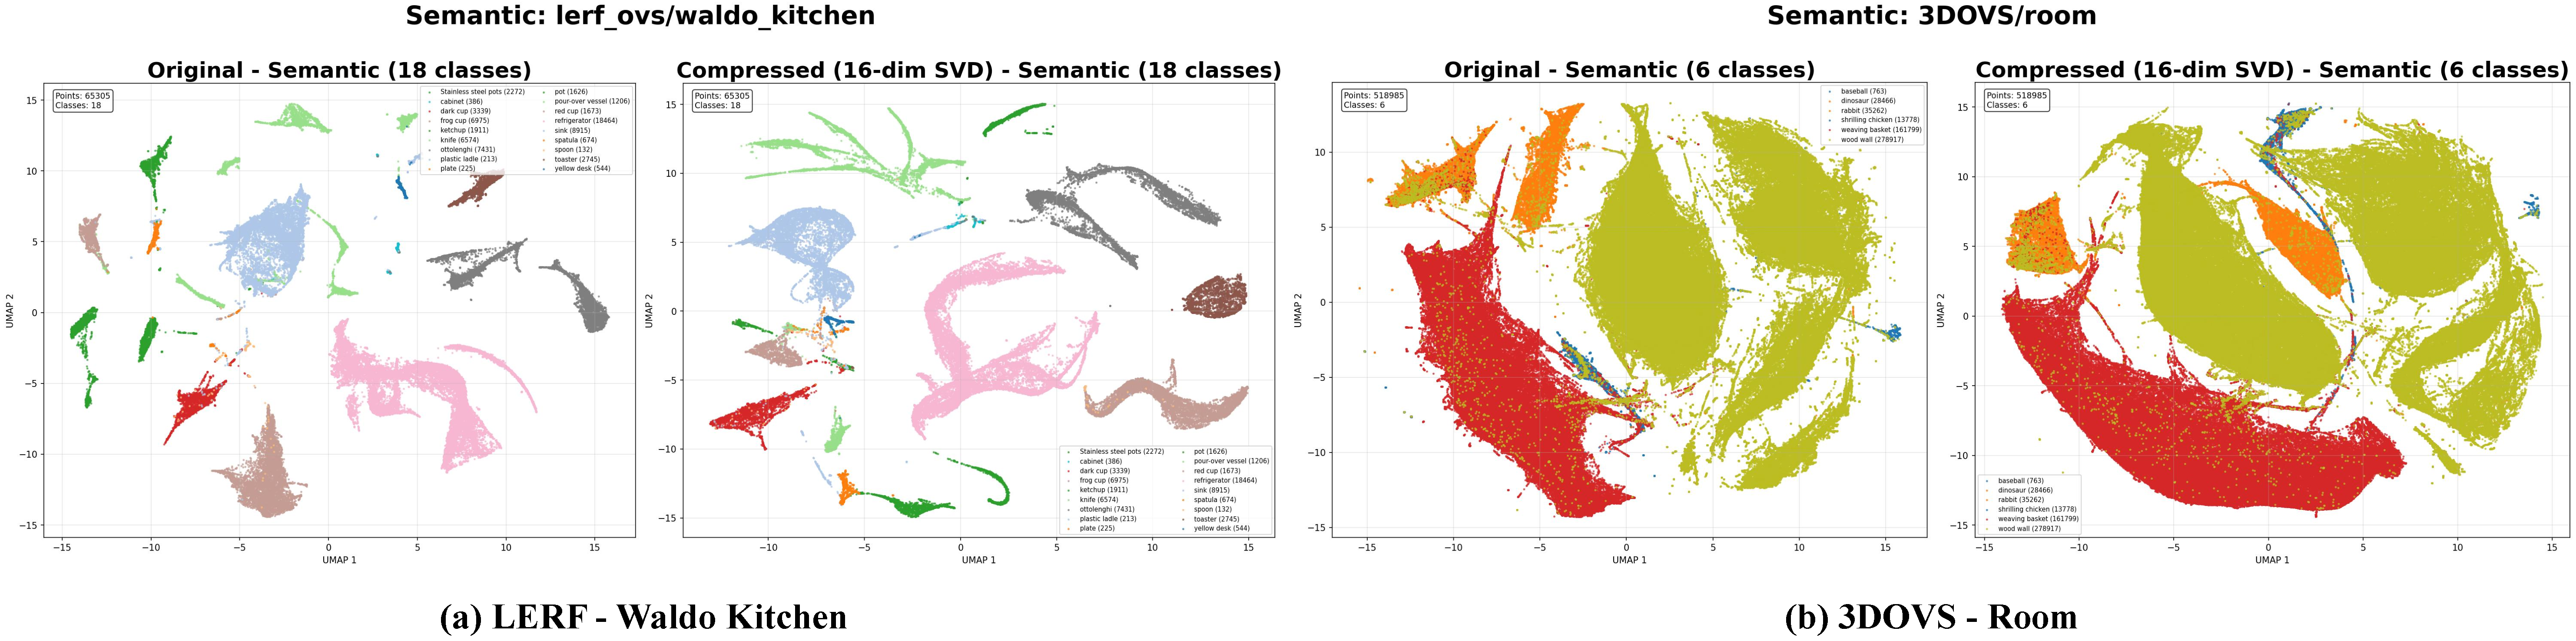
\includegraphics[width=\textwidth]{figs/JM-Visual.pdf}
  \caption{Visual comparison of feature distributions before and after dimensionality reduction in the feature space on the LERF and 3DOVS datasets.}
  \label{fig:JM-visual}
\end{figure}

\begin{table}[tb]
  \caption{Analysis of JM Distance. We present the JM distances computed under a Gaussian distribution assumption, as well as the JM distances obtained after aggregating the high‑dimensional distributions using arithmetic mean (AM) and geometric mean (GM). The compressed average JM distance actually shows an increasing trend.}
  \label{tab:jm-dist}
  \centering
  \resizebox{\textwidth}{!}{
  \begin{tabular}{@{}l|c|cccc|ccccc|c@{}}
    \toprule
    % 表头行：用 \multicolumn 覆盖竖线
    \multicolumn{1}{c}{\multirow{2}{*}{Setting}} & \multicolumn{1}{c}{\multirow{2}{*}{Metrics}} & \multicolumn{4}{c}{LERF} & \multicolumn{5}{c}{3D-OVS} & \multicolumn{1}{c}{\multirow{2}{*}{Avg}}\\
    \cmidrule(lr){3-6} \cmidrule(lr){7-11}
    \multicolumn{1}{c}{} & & Ramen & Figurines & Teatime & Kitchen & Bed & Bench & Room & Sofa & Lawn & \\
    \midrule
    & gaussian & 1.4128 & 1.4139 & 1.4110 & 1.4139 & 1.4142 & 1.4141 & 1.4142 & 1.4115 & 1.3875 & 1.4103\\
    origin & AM & 0.8061 & 0.9071 & 0.9522 & 0.9413 & 1.1786 & 1.0659 & 1.1303 & 1.1031 & 0.9342 & 1.0021\\
    & GM & 0.8506 & 0.9949 & 1.0322 & 1.0291 & 1.2492 & 1.1393 & 1.1987 & 1.1901 & 0.9702 & 1.0727\\
    \midrule
    & gaussian & 1.3887 & 1.4119 & 1.3994 & 1.4119 & 1.4142 & 1.4110 & 1.4137 & 1.4097 & 1.3013 & 1.3958($\textcolor{green}{-1.0\%}$)\\
    ours-16D & AM & 0.8992 & 1.0819 & 1.0661 & 1.1069 & 0.9475 & 1.0429 & 1.0045 & 1.0006 & 0.9539 & 1.0115($\textcolor{red}{+0.9\%}$)\\
    & GM & 0.9466 & 1.1829 & 1.1586 & 1.2319 & 1.1235 & 1.1397 & 1.1203 & 1.1649 & 0.9932 & 1.1179($\textcolor{red}{+4.2\%}$)\\
    \bottomrule
  \end{tabular}}
\end{table}

% 在这一节中，我们通过开放词汇场景领域常用的数据集，3DOVS与LERF数据集上的实验验证了SceneSplat-7k数据集中语言特征矩阵的低秩特性，并通过定量的方式验证了压缩后的特征空间的有效性。
In this section, we validate the low-rank property of the language feature matrix in the SceneSplat-7k \cite{li2025scenesplat} dataset through experiments on the commonly used open‑vocabulary scene datasets, namely 3DOVS \cite{liu2023weakly} and LERF\cite{lerf2023}, and quantitatively verify the effectiveness of the compressed feature space.

% 我们使用与SceneSplat相同的方法处理两个数据集，得到768维SigLIP2语言特征，并通过Occam's LGS聚合得到3D语言特征。随后，我们通过反投影的方式将2D标注映射到3DGS,并基于投票机制确定每个高斯的伪标签。我们使用UMap方法对原始特征空间和基于我们的方法压缩至16维的特征空间中各类别数据分布进行可视化，结果如图x所示。
% 压缩特征空间维度会细微影响各类别特征空间分布，但不影响类别间的可分性，原始高维空间中的不同簇在低维空间中亦不会重叠。
% Following the same procedure as in SceneSplat, we process both datasets to obtain 768‑dimensional SigLIP2 language features, which are then aggregated into 3D language features via Occam’s LGS \cite{cheng2024occamslgssimpleapproach}. The 2D annotations are subsequently back-projected onto the 3D Gaussians, and a voting mechanism is applied to assign pseudo‑labels to each Gaussian. We visualize the per‑class data distributions in the original feature space and in the 16‑dimensional feature space compressed by our method using UMAP, as shown in Figure \ref{fig:JM-visual}.
% While compressing the feature‑space dimension slightly alters the distribution of each class, it does not compromise inter‑class separability. The distinct clusters present in the original high‑dimensional space remain non‑overlapping after compression.
We follow SceneSplat’s procedure to process both datasets, extracting 768‑dim SigLIP2 \cite{tschannen2025siglip} language features and aggregating them into 3D language features via Occam’s LGS \cite{cheng2024occamslgssimpleapproach}. The 2D annotations are back‑projected onto 3D Gaussians, and a voting mechanism assigns pseudo‑labels to each Gaussian. In Figure \ref{fig:JM-visual}, we visualize the per‑class distributions in the original feature space and in our compressed 16‑dime space using UMAP.
Although feature‑space compression alters the within‑class distribution slightly, it preserves inter‑class separability: the distinct clusters observed in the original high‑dimensional space remain clearly separated after compression.

% 随后，我们使用JM距离对特征空间压缩前后各类别间的可分性进行定量分析。JM距离是一种衡量两个概率分布差异的距离度量，其值域为[0, √2]，值越大表示两类别的可分性越好。JM距离的定义基于巴氏距离，对于类别i,j，其概率分布$\tilde{p}_i(x)$与$\tilde{p}_j(x)}$间的巴氏距离为：
Subsequently, we employ the Jeffries-Matusita distance to quantitatively analyze the inter‑class separability before and after feature‑space compression. The JM distance, defined on the basis of the Bhattacharyya distance, measures the divergence between two probability distributions, ranging from 0 to $\sqrt{2}$, with larger values indicating better separability between two classes. The Bhattacharyya distance $B_{ij}$ between the probability distributions $\tilde{p}_i(x)$ and $\tilde{p}_j(x)$ is given by:
\begin{equation}
    B_{ij} = -\ln \left( \int \sqrt{\tilde{p}_i(x) \, \tilde{p}_j(x)} \, \mathrm{d}x \right)
\end{equation}
Hence, the JM distance between classes i and j is defined as $\text{JM}_{ij} = \sqrt{2(1 - e^{-B_{ij}})}$. We compute the average JM distance $\overline{\text{JM}}$ across all class pairs in a scene, where $c$ denotes the total number of classes.
\begin{equation}
    \overline{\text{JM}} = \frac{2}{c(c-1)} \sum_{i=1}^{c} \sum_{j>i}^{c} \sqrt{2(1 - e^{-B_{ij}})}
\end{equation}

% 实际计算过程中，需要先确定类别的分布以计算巴氏距离。当假设所有类别均为高斯分布时，类别i,j间的巴氏距离为：
To compute the Bhattacharyya distance in practice, the distribution of each class must first be estimated. Under the assumption that all classes follow Gaussian distributions, the Bhattacharyya distance between classes i and j is:
\begin{equation}
    B_{ij}^{\text{g}} = \frac{1}{8} (\mathbf{M}_i - \mathbf{M}_j)^T \left( \frac{\mathbf{V}_i + \mathbf{V}_j}{2} \right)^{-1} (\mathbf{M}_i - \mathbf{M}_j) + \frac{1}{2} \ln \left( \frac{ | \frac{\mathbf{V}_i + \mathbf{V}_j}{2} | }{ \sqrt{ | \mathbf{V}_i | \cdot | \mathbf{V}_j | } } \right)
\end{equation}
where $\mathbf{M}_i$ and $\mathbf{M}_j$ are the mean vectors of classes i and j, respectively, and $\mathbf{V}_i$ and $\mathbf{V}_j$ are their corresponding covariance matrices.
% 然而，所有类别不一定都满足高斯分布。同时，基于高斯分布假设计算JM距离时，高维特征的JM距离理论上大于低维特征，因为每个独立维度都为Bhattacharyya距离贡献非负值，产生累积的"维度红利"效应。因此，我们使用离散化方式计算任意分布间的JM距离。
% 具体而言，对每个维度的特征值进行离散化分箱统计得到各维度直方图，计算每维度的Bhattacharyya系数后通过算术/几何平均聚合，最后转换为JM距离。采用平均聚合的原因是各维度一般不满足相互独立，通过按维度平均的策略避免维度红利。基于算术和几何平均聚合的JM距离计算公式分别如Eq25,Eq26。
% However, not all classes necessarily follow Gaussian distributions. Moreover, when computing JM distances under the Gaussian assumption, the distance for high‑dimensional features is theoretically greater than that for low‑dimensional ones, because each independent dimension contributes a non‑negative value to the Bhattacharyya distance, resulting in a cumulative ``dimensional bonus'' effect. Therefore, we compute JM distances between arbitrary distributions using a discretization approach.
% Specifically, the feature values in each dimension are discretized into bins to obtain per‑dimensional histograms. The Bhattacharyya coefficient is computed for each dimension and then aggregated via arithmetic or geometric averaging, after which it is converted to  JM distance. Averaging across dimensions is adopted because the dimensions are generally not independent. This strategy avoids the dimensional bonus effect. 
Not all classes follow Gaussian distributions, and under the Gaussian assumption, high‑dimensional features obtain artificially inflated JM distances because each independent dimension adds a non‑negative contribution—a “dimensional‑bonus” effect. To avoid this, we compute JM distances via discretization. We bin the feature values in each dimension, compute the Bhattacharyya coefficient per dimension, aggregate the coefficients by arithmetic or geometric averaging, since dimensions are generally correlated, and finally convert the result to JM distance. This procedure makes no Gaussian or independence assumptions and eliminates the dimensional bonus.
The formulas for the JM distance based on arithmetic and geometric‑mean aggregation are given in Eq.\eqref{eq:jmam} and Eq.\eqref{eq:jmgm}, respectively.
\begin{equation}
    \text{JM}_{ij}^{\text{AM}} = \sqrt{2 \left(1 - \frac{1}{D} \sum_{d=1}^{D} \sum_{k=1}^{n_{b}} \sqrt{\tilde{p}_i(d,k) \cdot \tilde{p}_j(d,k)}\right)} 
    \label{eq:jmam}
\end{equation}
\begin{equation}
    \text{JM}_{ij}^{\text{GM}} = \sqrt{2 \left(1 - \exp\left(\frac{1}{D} \sum_{d=1}^{D} \ln\left(\sum_{k=1}^{n_{b}} \sqrt{\tilde{p}_i(d,k) \cdot \tilde{p}_j(d,k)}\right)\right)\right)}
    \label{eq:jmgm}
\end{equation}
where $n_b$ denotes the number of bins in the histogram, and $D$ indicates the feature dimensionality. 
% 各场景3种平均JM距离如表2所示。使用我们的方法压缩至16维的特征空间，其平均JM距离甚至整体高于原始特征空间，这证明了原始特征矩阵的冗余性。即使在高度压缩的低维空间中，不同类别特征分布间依然能保持良好的可分性，因此在不损失分类性能前提下进行降维是可能的。
The average JM distances across scenarios for different aggregation methods are presented in Table \ref{tab:jm-dist}. Our 16‑dimensionally compressed feature space yields an even higher average JM distance than the original space, confirming the redundancy of the original feature matrix. The distinct classes remain well‑separable in this low‑dimensional space, demonstrating that dimensionality reduction can be achieved without degrading classification performance.


\section{Details of Experimental Setup}
\label{sec:exp_details}

\subsection{Dataset Splits and Evaluation Details}

\noindent\textbf{SceneSplat-7k.} We evaluate our method on SceneSplat-7K, a large-scale indoor benchmark comprising 7,916 high-fidelity 3DGS scenes~\cite{dai2017scannet, yeshwanth2023scannet++, straub2019replica, roberts2021hypersim, wald20193rscan, dehghan2021arkitscenes, chang2017matterport3d}. Following its protocol, we pretrain on 4,114 scenes from ScanNet, ScanNet++ v2, and Matterport3D, and evaluate on their respective test sets across diverse object scales. We report average foreground IoU and accuracy.

\noindent\textbf{LERF-OVS.} Quantitative evaluations are conducted on the LERF-OVS dataset, which comprises everyday indoor scenes featuring diverse objects with pixel-wise semantic masks and paired short text queries. Adhering to the standard LERF evaluation protocol~\cite{lerf2023}, we focus on four representative scenes: Ramen, Figurines, Teatime, and Waldo Kitchen. Performance is assessed using two key metrics: mean IoU for open-vocabulary segmentation and localization accuracy.

% \noindent\textbf{LERF-MASK.} The LERF-Mask benchmark~\cite{ye2024gaussian}, a semantic subset of the original LERF dataset~\cite{lerf2023}, serves as the foundation for our evaluation. Comprising three indoor scenes (Figures, Ramen, and Teatime) annotated with 23 text prompts and 6--10 dense object masks per scene, this benchmark facilitates precise open-vocabulary segmentation assessment. Following~\cite{ye2024gaussian,lyu2024gaga}, we assess performance using mean Intersection over Union (mIoU) and boundary IoU (mBIoU).

% \noindent\textbf{3DOVS.} Evaluation of our method is also conducted on the 3D-OVS dataset \cite{liu2023weakly}, which features long-tail objects situated in diverse backgrounds. Following the protocol established in Occam's LGS \cite{cheng2024occamslgssimpleapproach}, we employ a dynamic thresholding strategy to identify and evaluate only stable regions. Quantitative assessment is conducted on five representative scenes: Sofa, Lawn, Bed, Room, and Bench. We utilize the ground-truth annotations provided by \cite{qin2024langsplat} to measure segmentation performance for these scenes.

% \noindent\textbf{Replica.}
% The Replica dataset~\cite{replica19arxiv} offers high-fidelity indoor reconstructions with dense geometry and comprehensive ground-truth annotations. Following the protocol in~\cite{Zhi:etal:ICCV2021,lyu2024gaga}, we select eight scenes and utilize their provided rendered imagery. For each scene, we uniformly split the data into 20\% for training and 20\% for testing, yielding 180 images per set. To evaluate the multi-view consistency of 3D segmentation masks, we leverage the dataset's ground-truth panoptic labels, disregarding specific class semantics.

% 我们的方法默认使用16-dim的特征进行训练，并报告指标。
\noindent\textbf{Note.} By default, our method employs \textbf{16-dim} features for training and reports the corresponding metrics.
\subsection{Implementation Details}
% SceneSplat使用PTv3作为基础模型进行基于3DGS的Vision-Language Pretraining。由于我们对特征进行了大幅度降维，因此可以使用更小，更轻量化的模型预测低维度的语言特征参数。我们使用LitePT作为基础模型，冻结其编码器并修改解码器架构以适配更低维度的输出。同时，我们也实现了一个基于PTv3的，仅修改解码器特征维度的版本。模型详细架构分别如表1和2所示，我们将在Sec.\ref{}进行详细消融实验。
SceneSplat employs PTv3 \cite{wu2024ptv3} as the backbone for 3DGS-based vision-language pretraining. Given our significant reduction in feature dimensionality, we can leverage smaller, more lightweight models to predict these low-dimensional language feature parameters. Specifically, we utilize LitePT \cite{yuelitept2026} as the backbone, freezing its encoder while modifying the decoder architecture to accommodate the lower-dimensional output. Additionally, we implement a variant based on PTv3 that modifies only the decoder's feature dimensionality. The detailed model architectures are presented in Table \ref{tab:litept} and \ref{tab:ptv3}, with comprehensive ablation studies provided in Section \ref{sec:ablation_details}.

We optimize all parameters of the 3D Gaussian primitives, including center position, color, opacity, quaternion rotation, and scale. The model is trained using the AdamW optimizer (initial learning rate $0.001$, weight decay $0.05$) coupled with a OneCycle scheduler featuring cosine annealing. Our objective function combines cosine similarity ($\lambda_{cos}=0.1$), L1 regularization ($\lambda_{L1}=1.0$), density consistency regularization ($\lambda_{dense}=1.0$)and contrastive loss ($\lambda_{con}=0.02$, temperature $\tau=0.2$). Notably, the contrastive loss is activated only during the final 75\% of the training process. To enhance robustness, we employ extensive data augmentation strategies, including random rotations, scaling, flipping, jittering, and elastic distortions.

% 我们使用4个RTX4090 GPU进行800轮data epochs训练。所有代码均基于PyTorch框架实现。
Training is conducted for 800 data epochs on four NVIDIA RTX 4090 GPUs. All inference experiments are conducted on a single NVIDIA RTX 4090. All implementations are built upon the PyTorch framework.

% 需要注意的是，针对2D评估标准，为了与SceneSplat方法进行公平比较，我们遵循官方提供的数据预处理流程基于训练视图提取768维度的siglip2-sam2语言特征，并统一进行10 epoch的微调。其余方法均使用512维CLIP特征，因此与我们的方法不能进行直接的比较，我们主要以SceneSplat为参考。
It is important to note that for the 2D evaluation metrics, we strictly adhere to the official data preprocessing pipeline of SceneSplat to ensure a fair comparison. Specifically, we extract 768-dimensional \textbf{SigLIP2-SAM2} language features from the training views. Since other baseline methods typically employ 512-dimensional CLIP features, direct comparison with them is not feasible due to the feature dimension mismatch. Consequently, our primary benchmark for evaluation is SceneSplat.

\begin{table}[htbp]
    \centering
    % PTv3
    \begin{minipage}[t]{0.5\textwidth}
    \caption{Model Configs for LitePT Vision-Language Pretraining.}
    \label{tab:litept}
    \resizebox{1\linewidth}{!}{
    \begin{tabular}{l|l}
    \toprule
    Config & Value \\
    \midrule
    embedding depth & 2 \\
    embedding channels & 32 \\
    encoder depth & [2, 2, 2, 6, 2] \\
    encoder channels & [36, 72, 144, 252, 504] \\
    encoder num heads & [2, 4, 8, 14, 28] \\
    encoder patch size & [1024, 1024, 1024, 1024, 1024] \\
    decoder depth & [2, 2, 2, 2] \\
    decoder channels & [16, 32, 64, 126] \\
    decoder num heads & [1, 2, 4, 7] \\
    decoder patch size & [1024, 1024, 1024, 1024] \\
    down stride & $[\times 2, \times 2, \times 2, \times 2, \times 2]$ \\
    mlp ratio & 2 \\
    qkv bias & True \\
    drop path & 0.3 \\
    \bottomrule
    \end{tabular}}
    \end{minipage}%
    \hfill%
    % 针对高维语言特征的不同适配与对齐方法在显存消耗与用时方面的对比。
    \begin{minipage}[t]{0.48\textwidth}%
    \caption{Model Configs for PTv3 Vision-Language Pretraining.}
    \label{tab:ptv3}
    \resizebox{1\linewidth}{!}{
    \begin{tabular}{l|l}
    \toprule
    Config & Value \\
    \midrule
    embedding depth & 2 \\
    embedding channels & 32 \\
    encoder depth & [2, 2, 2, 6] \\
    encoder channels & [32, 64, 128, 256] \\
    encoder num heads & [2, 4, 8, 16] \\
    encoder patch size & [1024, 1024, 1024, 1024] \\
    decoder depth & [2, 2, 2] \\
    decoder channels & [16, 64, 256] \\
    decoder num heads & [8, 8, 8] \\
    decoder patch size & [1024, 1024, 1024] \\
    down stride & $[\times 2, \times 2, \times 2, \times 2]$ \\
    mlp ratio & 2 \\
    qkv bias & True \\
    drop path & 0.3 \\
    \bottomrule
    \end{tabular}}
    \end{minipage}
\end{table}
% ---------------------------------------------------------------
% Section C: Additional Comparisons
% ---------------------------------------------------------------
% \section{Additional Comparison Results}
% \label{sec:add_comparisons}

\iffalse
\begin{table}[htbp]
\caption{Comparison of average IoU and F1 score on Replica Dataset.}
\begin{center}
\begin{tabular}{l|c|c|cc|c}
\toprule
Method & Venue & Type & mIoU(\%) & F-score (\%) & Time \\
\midrule
% LERF \cite{lerf2023} & ICCV'23 & Per-scene Optimization & 37.2 & 29.3 & >1h\\
% LangSplat \cite{qin2024langsplat} & CVPR'24 & Per-scene Optimization & 57.6 & 53.6 & >1h\\
Gaga \cite{lyu2024gaga} & Arxiv'24 & Semantic Clustering & 46.2 & 44.4 & 8min\\ %8.11min
GS-Grouping \cite{ye2024gaussian} & ECCV'24 & Semantic Clustering & 23.6 & 30.4 & >2h\\
OmniSeg3D-GS \cite{ying2023omniseg3d} & CVPR'24 & Per-scene Optimization & 39.1 & 35.9 & 20min\\ %20.35min
Unified-Lift \cite{zhu2025rethinking}& CVPR'25 & Per-scene Codebook & 41.6 & 43.9 & >2h\\

\midrule
SceneSplat* \cite{li2025scenesplat}& ICCV'25 & Generalizable & 40.1 & 40.3 & \underline{0.36min}\\
Ours & - & Generalizable & - & - & \textbf{0.06min}\\
\bottomrule
\end{tabular}
\label{tab: LERF}
\end{center}
\end{table}

\begin{table}[htbp]
\caption{Comparison of average IoU on 3D-OVS Dataset.}
\begin{center}
\resizebox{\textwidth}{!}{
\begin{tabular}{l|c|ccccc|c|c}
\toprule
Methods & Type & Bed & Bench & Room & Sofa & Lawn & Overall & Time\\
\midrule
% \specialrule{0.4pt}{0pt}{0pt} 
% LSeg & 56.0 & 6.0 & 19.2 & 4.5 & 17.5 & 20.6 \\
% LERF & 73.5 & 53.2 & 46.6 & 27.0 & 73.7 & 54.8 \\
GS-Grouping \cite{ye2024gaussian}& Semantic Clustering & 83.0 & 91.5 & 85.9 & 87.3 & 90.6 & 87.7 & >2h\\
Feature-3DGS \cite{zhou2024feature}& Per-scene Optimization & 83.5 & 90.7 & 84.7 & 86.9 & 93.4 & 87.8 & >3h\\
LEGaussians \cite{shi2024language}& Per-scene Optimization & 84.9 & 91.1 & 86.0 & 87.8 & 92.5 & 88.5 & >3h\\
GOI \cite{qu2024goi}& Per-scene Codebook & 89.4 & 92.8 & 91.3 & 85.6 & 94.1 & 90.6 & 45min\\
ILGS \cite{jsmbankILGS}& Per-scene Optimization & 96.4 & 95.5 & 93.6 & 92.2 & 94.2 & \underline{94.4} & 50min\\
LangSplat \cite{qin2024langsplat}& Per-scene Optimization & 92.5 & 94.2 & 94.1 & 90.0 & 96.1 & 93.4 & >1h\\
OccamLGS \cite{cheng2024occamslgssimpleapproach}& Per-scene Optimization-Free & 96.8 & 95.8 & 96.5 & 88.8 & 97.0 & \textbf{95.0} & 2min\\
\midrule
SceneSplat* \cite{li2025scenesplat}& Generalizable & 88.4 & 92.7 & 93.7 & 86.7 & 93.9 & 91.1 & \underline{0.22min}\\
Ours & Generalizable & 90.5 & 94.1 & 91.3 & 89.4 & 95.0 & 92.1 & \textbf{0.04min}\\
\bottomrule
\end{tabular}}
\label{tab: 3DOVS}
\end{center}
\end{table}
\fi

\iffalse
\begin{table}[tb]
  \centering
  \caption{Quantitative comparisons with generalized methods on [Dataset].}
  \label{tab:supp_comp_llff}
  \begin{tabular}{l c c c c}
    \toprule
    \textbf{Method} & \textbf{Setting} & \textbf{PSNR $\uparrow$} & \textbf{SSIM $\uparrow$} & \textbf{LPIPS $\downarrow$} \\
    \midrule
    Method A~\cite{RefA} & Pre-trained & 12.34 & 0.250 & 0.591 \\
    Method A~\cite{RefA} & Fine-tuned  & 17.07 & 0.436 & 0.529 \\
    Method B~\cite{RefB} & Pre-trained & 7.93  & 0.272 & 0.682 \\
    \textbf{Ours}        & \textbf{Sparse-view} & \textbf{20.45} & \textbf{0.712} & \textbf{0.196} \\
    \bottomrule
  \end{tabular}
\end{table}
\fi

% ---------------------------------------------------------------
% Section D: Ablation Studies Details
% ---------------------------------------------------------------
\section{Additional Ablation Results}
\label{sec:ablation_details}
\label{sec:extended-ablation}
\begin{table}[tb]
  \centering
  \caption{RPCA ablations on LERF.}
  \label{tab:ablation_latency}
  \begin{tabular}{@{}l|cc@{}}
    \toprule
    Method & Error & Latency \\
    \midrule
    RPCA-CPU & $6.28 \times 10^{-6}$ & >2h \\
    RPCA-GPU & $6.28 \times 10^{-6}$ & 330.55s \\
    Structured RPCA & $9.37 \times 10^{-3}$ & 0.18s \\
    \bottomrule
  \end{tabular}
\end{table}
\begin{table}[tb]
  \centering
  \caption{Ablation study on model architecture. We report the supervised semantic segmentation performance on ScanNet20.}
  \label{tab:ablation-arch}
  \begin{tabular}{c|cc|cc}
    \toprule
    \textbf{Model} &  mIoU(\%) & mAcc (\%) & Params(M) & Inference Time \\
    \midrule
    SceneSplat & 77.2 & 84.6 & 91.72 & 0.16min \\
    \midrule
    Ours-PTv3 & 77.2 & 84.5 & \underline{20.99} & \underline{0.05min} \\
    Ours-LitePT & 77.0 & 84.3 & \textbf{9.58} & \textbf{0.03min} \\
    \bottomrule
  \end{tabular}
\end{table}

We provide comprehensive ablation studies regarding efficiency, architectural choices and input
densities that could not be included in the main paper due to space constraints.

\subsection{Ablations on Model Architecture}
% 如表3所示，我们在ScanNet数据集上分别对LitePT与PTv3两种架构进行了有监督语义分割的性能评估。使用LitePT的版本相比PTv3版本在性能上不会有很大差距，却有着更小的参数量和更快的推理速度。虽然使用LitePT是最优选择，使用PTv3相比baseline依旧实现了4倍的参数量减小和3倍的推理加速。这说明了我们的语言特征压缩方法的有效性。
As shown in Table \ref{tab:ablation-arch}, we evaluate the supervised semantic segmentation performance of both LitePT and PTv3 architectures on the ScanNet dataset. The LitePT variant achieves performance comparable to PTv3, yet with significantly fewer parameters and faster inference speeds. While LitePT represents the optimal choice, the PTv3 variant still delivers a 4-fold reduction in parameters and a 3-fold acceleration in inference compared to the baseline. These results underscore the effectiveness of our language feature compression method.

\subsection{Ablations on input densities}
% 我们在ScanNet200上进行消融实验，以说明我们方法针对不同密度输入的鲁棒性。我们按照不同比例对原始3DGS进行下采样后输入模型，得到稀疏的3D语言特征，随后基于近邻投票策略进行0样本3D分割。随着采样率逐渐降低，整体性能成下降趋势，这是因为下采样一定程度上破坏了局部的几何结构和语义信息。而我们的Density Invariant learning策略相比不应用时在稀疏输入下有明显的性能提升，这说明了我们方法对稀疏输入的鲁棒性。
We conduct ablation studies on the ScanNet200 dataset in Table \ref{tab:sample-ablation} to demonstrate the robustness of our method against inputs of varying densities. Specifically, we downsample the original 3DGS at various ratios to generate sparse 3D language features, which are then processed via a nearest-neighbor voting strategy for zero-shot 3D segmentation.
In this paper, we set $K=3$, corresponding to the three sampling scenarios used in the density consistency loss: dense, half-density, and single-point-per-grid inputs.
As the sampling rate decreases, overall performance exhibits a downward trend, which is consistent with downsampling partially disrupting local geometric structures and semantic information. However, compared to the baseline without our Density-Invariant Learning strategy, our approach yields consistent improvements under sparse input conditions. The gains are modest at moderate compression levels but remain directionally stable across the sampling settings we evaluate, suggesting improved robustness when handling sparse data.


\begin{table}[htbp]
    \centering
    % Scannet 数据集上针对不同采样设置下，不同密度输入下性能的消融。
    \begin{minipage}[t]{0.5\textwidth}
    \caption{Ablation study on performance under different sampling settings and input densities on the ScanNet200 benchmark.}
    \label{tab:sample-ablation}
    \resizebox{1\linewidth}{!}{
    \begin{tabular}{c|cc|cc}
    \toprule
    \multirow{2}{*}{\textbf{Sample Rate}} & \multicolumn{2}{c}{with $\mathcal{L}_{dense}$} & \multicolumn{2}{c}{w/o $\mathcal{L}_{dense}$} \\
    \cmidrule(lr){2-3} \cmidrule(lr){4-5}
    & mIoU & mAcc & mIoU & mAcc \\
    \midrule
    30$\%$ & 18.0 & 30.6 & 16.0 & 29.1\\
    50$\%$ & 18.5 & 31.2 & 17.2 & 30.0\\
    70$\%$ & 18.8 & 31.7 & 18.0 & 30.7\\
    100$\%$ & 19.0 & 31.9 & 18.4 & 31.2\\
    \bottomrule
    \end{tabular}}
    \end{minipage}%
    \hfill%
    % 针对高维语言特征的不同适配与对齐方法在显存消耗与用时方面的对比。
    \begin{minipage}[t]{0.48\textwidth}%
      \caption{Comparison of memory consumption and runtime for different adaptation and alignment methods targeting high-dimensional language features.}
      \label{tab:efficiency}
      \resizebox{1\linewidth}{!}{
      \begin{tabular}{c|cc}
        \toprule
        \textbf{Method} & GPU Mem(MB) & Time \\
        \midrule
        Auto Encoder & 494 & 1h \\
        \midrule
        Ours-8dim & \textbf{165} & \textbf{5.7ms} \\
        Ours-16dim & \underline{297}& \underline{8.4ms} \\
        Ours-32dim & 563 & 14.5ms \\
        \bottomrule
      \end{tabular}}
    \end{minipage}
\end{table}

% 不同维度空间对齐方法的效率比较 Dimensional Space
\subsection{Efficiency Comparison of Different Alignment Methods}
% 以往基于CLIP等2D预训练模型的方法，在对原始高维语言特征进行降维时，不可避免的需要依赖每个场景训练一个Auto Encoder，以压缩和恢复特征，这个过程十分漫长。而我们的Orthogonal Procrustes Analysis方法仅需求解一个低维的变换矩阵，便可直接将高维文本嵌入与低维特征对齐。具体计算与存储开销见表5，我们的方法每场景仅需毫秒级别的开销，相比Auto Encoder快了6个数量级，同时占用更少内存。使用我们的方法可以几乎无损耗的在低维空间实现推理，使实时的3D开放词汇感知与场景理解成为可能。
Previous methods \cite{cheng2024occamslgssimpleapproach, qin2024langsplat, li2025langsplatv2} based on 2D pre-trained models like CLIP \cite{DBLP:journals/corr/abs-2103-00020} often require training a scene-specific autoencoder to compress and reconstruct high-dimensional language features during dimensionality reduction. In contrast, our Orthogonal Procrustes Analysis approach only requires solving for a low-dimensional transformation matrix to directly align high-dimensional text embeddings with low-dimensional features.
As detailed in Table \ref{tab:efficiency}, our method incurs millisecond-level overhead per scene and consumes less memory than the autoencoder-based alternative. This alignment cost is incurred only at query time, whereas constructing SceneSplat-Compact itself is a one-time offline preprocessing step that can be amortized across repeated downstream runs. The result makes low-dimensional inference practical without the per-scene optimization burden of autoencoder-based reduction.


% ---------------------------------------------------------------
% Section E: Visualizations
% ---------------------------------------------------------------
\section{Additional Visualization Results}
\label{sec:add_vis}

\subsection{Comparison with SOTA Methods}
% 图1展示了我们方法在3DOVS与Replica数据集上的零样本开放词汇物体定位与实例分割的结果。我们的方法与SceneSplat有着相当的泛化性能。
Figure \ref{fig:SuppVisualize} illustrates the results of our method for zero-shot open-vocabulary object localization and instance segmentation on the 3DOVS\cite{liu2023weakly} and Replica\cite{straub2019replica} datasets. Our approach demonstrates comparable generalization performance to SceneSplat.

\subsection{Visualizations of Our Method}
% 图2展示了Scannet数据集上特征图在降维前后的PCA可视化对比。降维前后基本不损失空间和语义信息，只是在可视化的时候存在颜色差异，这是由PCA本身的性质决定的。
Figure \ref{fig:Visualize-Compare} presents a PCA visualization comparison of feature maps on the ScanNet dataset before and after dimensionality reduction. The low-dimensional representation preserves most of the large-scale spatial and semantic structure, although some fine-grained boundaries and closely related categories become less distinct. The observed color discrepancies in the visualization are also affected by the nature of PCA itself.

\begin{figure}[tb]
  \centering
  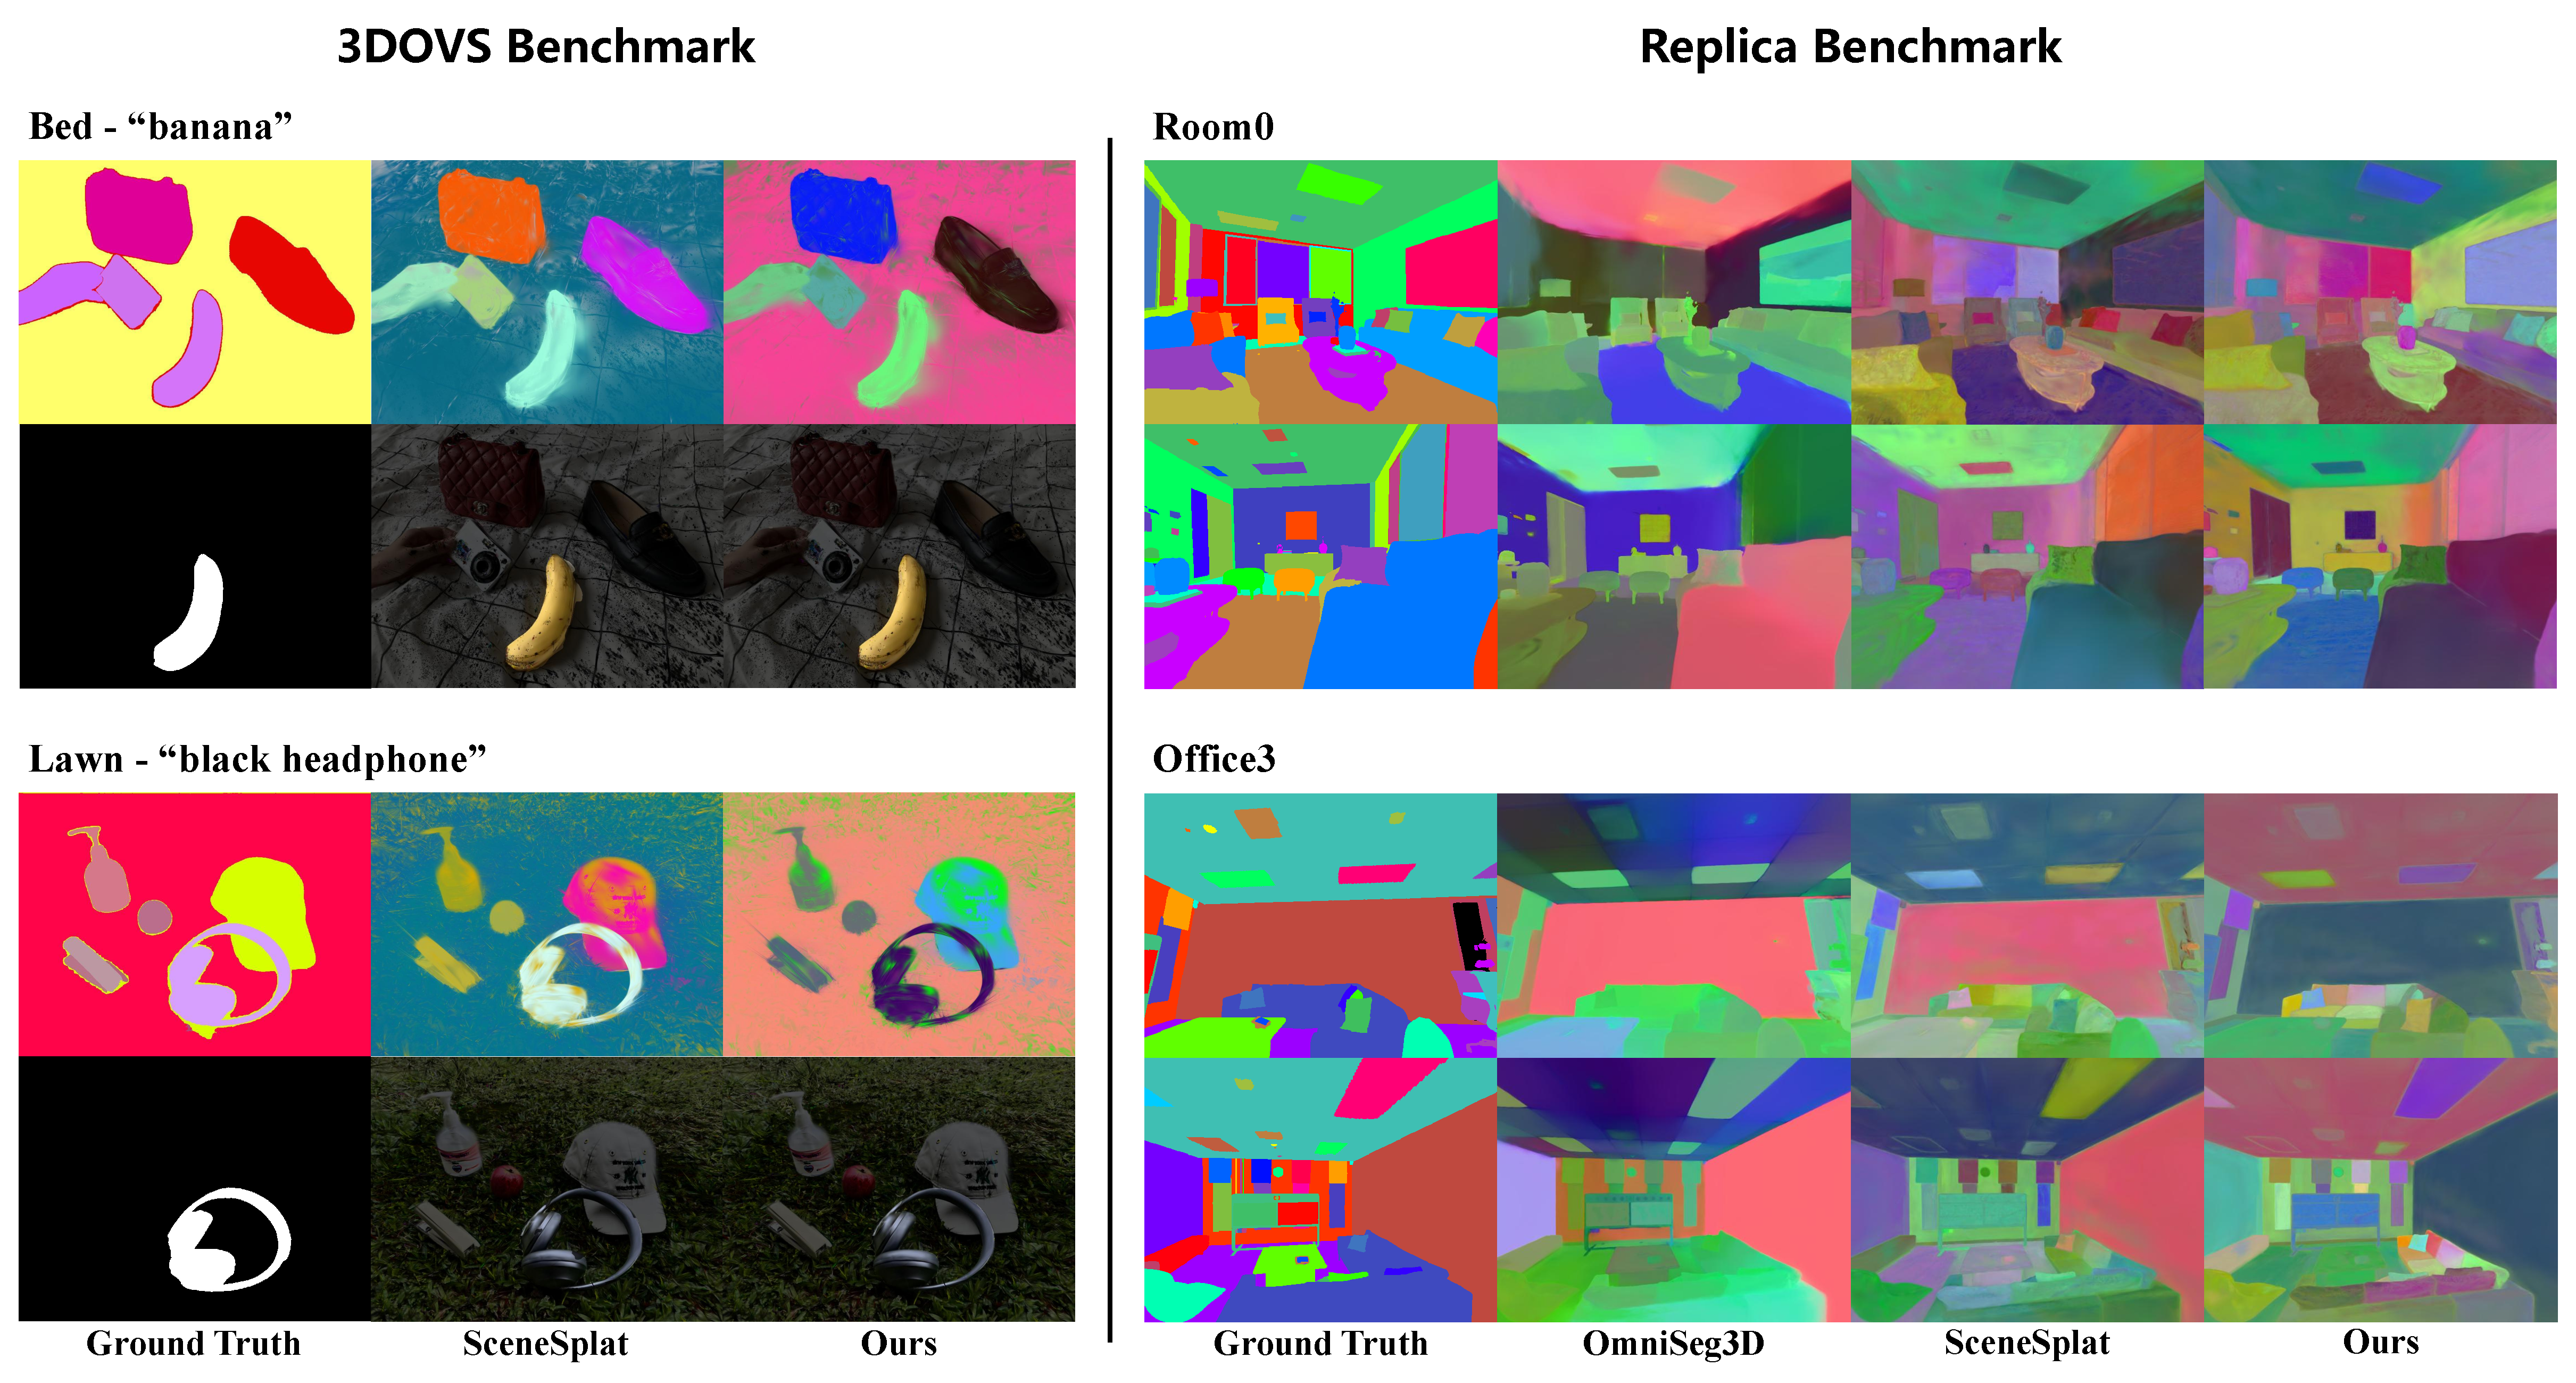
\includegraphics[width=\textwidth]{figs/Replica-3DOVS.pdf}
  \caption{Visualization of open-vocabulary recognition and object query results on the 3DOVS \& Replica datasets. Our model demonstrates strong generalization capabilities.}
  \label{fig:SuppVisualize}
\end{figure}

% ---------------------------------------------------------------
% Section F: Future Work
% ---------------------------------------------------------------
\section{Discussion, Limitations, and Future Work}
\label{sec:future}
While our compression pipeline achieves substantial storage reduction and fast inference, we observe several important limitations. First, optimizing models in the compressed low-dimensional space is more difficult than in the original high-dimensional setting: convergence is slower, sensitivity to hyperparameters is higher, and the simplified representation may blur difficult boundaries or fine-grained categories. This suggests that the current linear projection, while efficient for alignment and deployment, does not fully preserve the optimization geometry of the original feature space.

Second, our empirical study is centered on the storage bottleneck caused by large precomputed language features in SceneSplat-style pipelines. Although the underlying ideas may transfer more broadly, the paper does not claim universal gains across all 3D open-vocabulary representations, feature encoders, or training recipes. Third, the strongest benefit of our method is efficiency; under aggressive compression, absolute accuracy can still lag behind heavier methods that optimize directly in the original feature space. Finally, we do not exhaustively ablate the grid size used in spatial aggregation. This parameter controls a trade-off between stronger compression and better preservation of boundaries, small objects, and rare categories, and a more systematic sensitivity study is left to future work.

Future work will focus on discovering more training-friendly low-dimensional feature transformations. We also plan to report the end-to-end cost of constructing SceneSplat-Compact more systematically at larger scales and to study stronger baselines for feature extraction-time compression. In addition, we will investigate learnable non-linear mapping functions or adaptive basis expansions that can better preserve the optimization geometry of the original features while maintaining compactness. Exploring network architectures specifically tailored for low-dimensional feature training could further mitigate the difficulty of optimization in compressed spaces. By designing structures that better align with the geometric properties of the reduced latent space, we aim to ultimately bridge the gap between extreme compression efficiency and training stability.

\begin{figure}[tb]
  \centering
  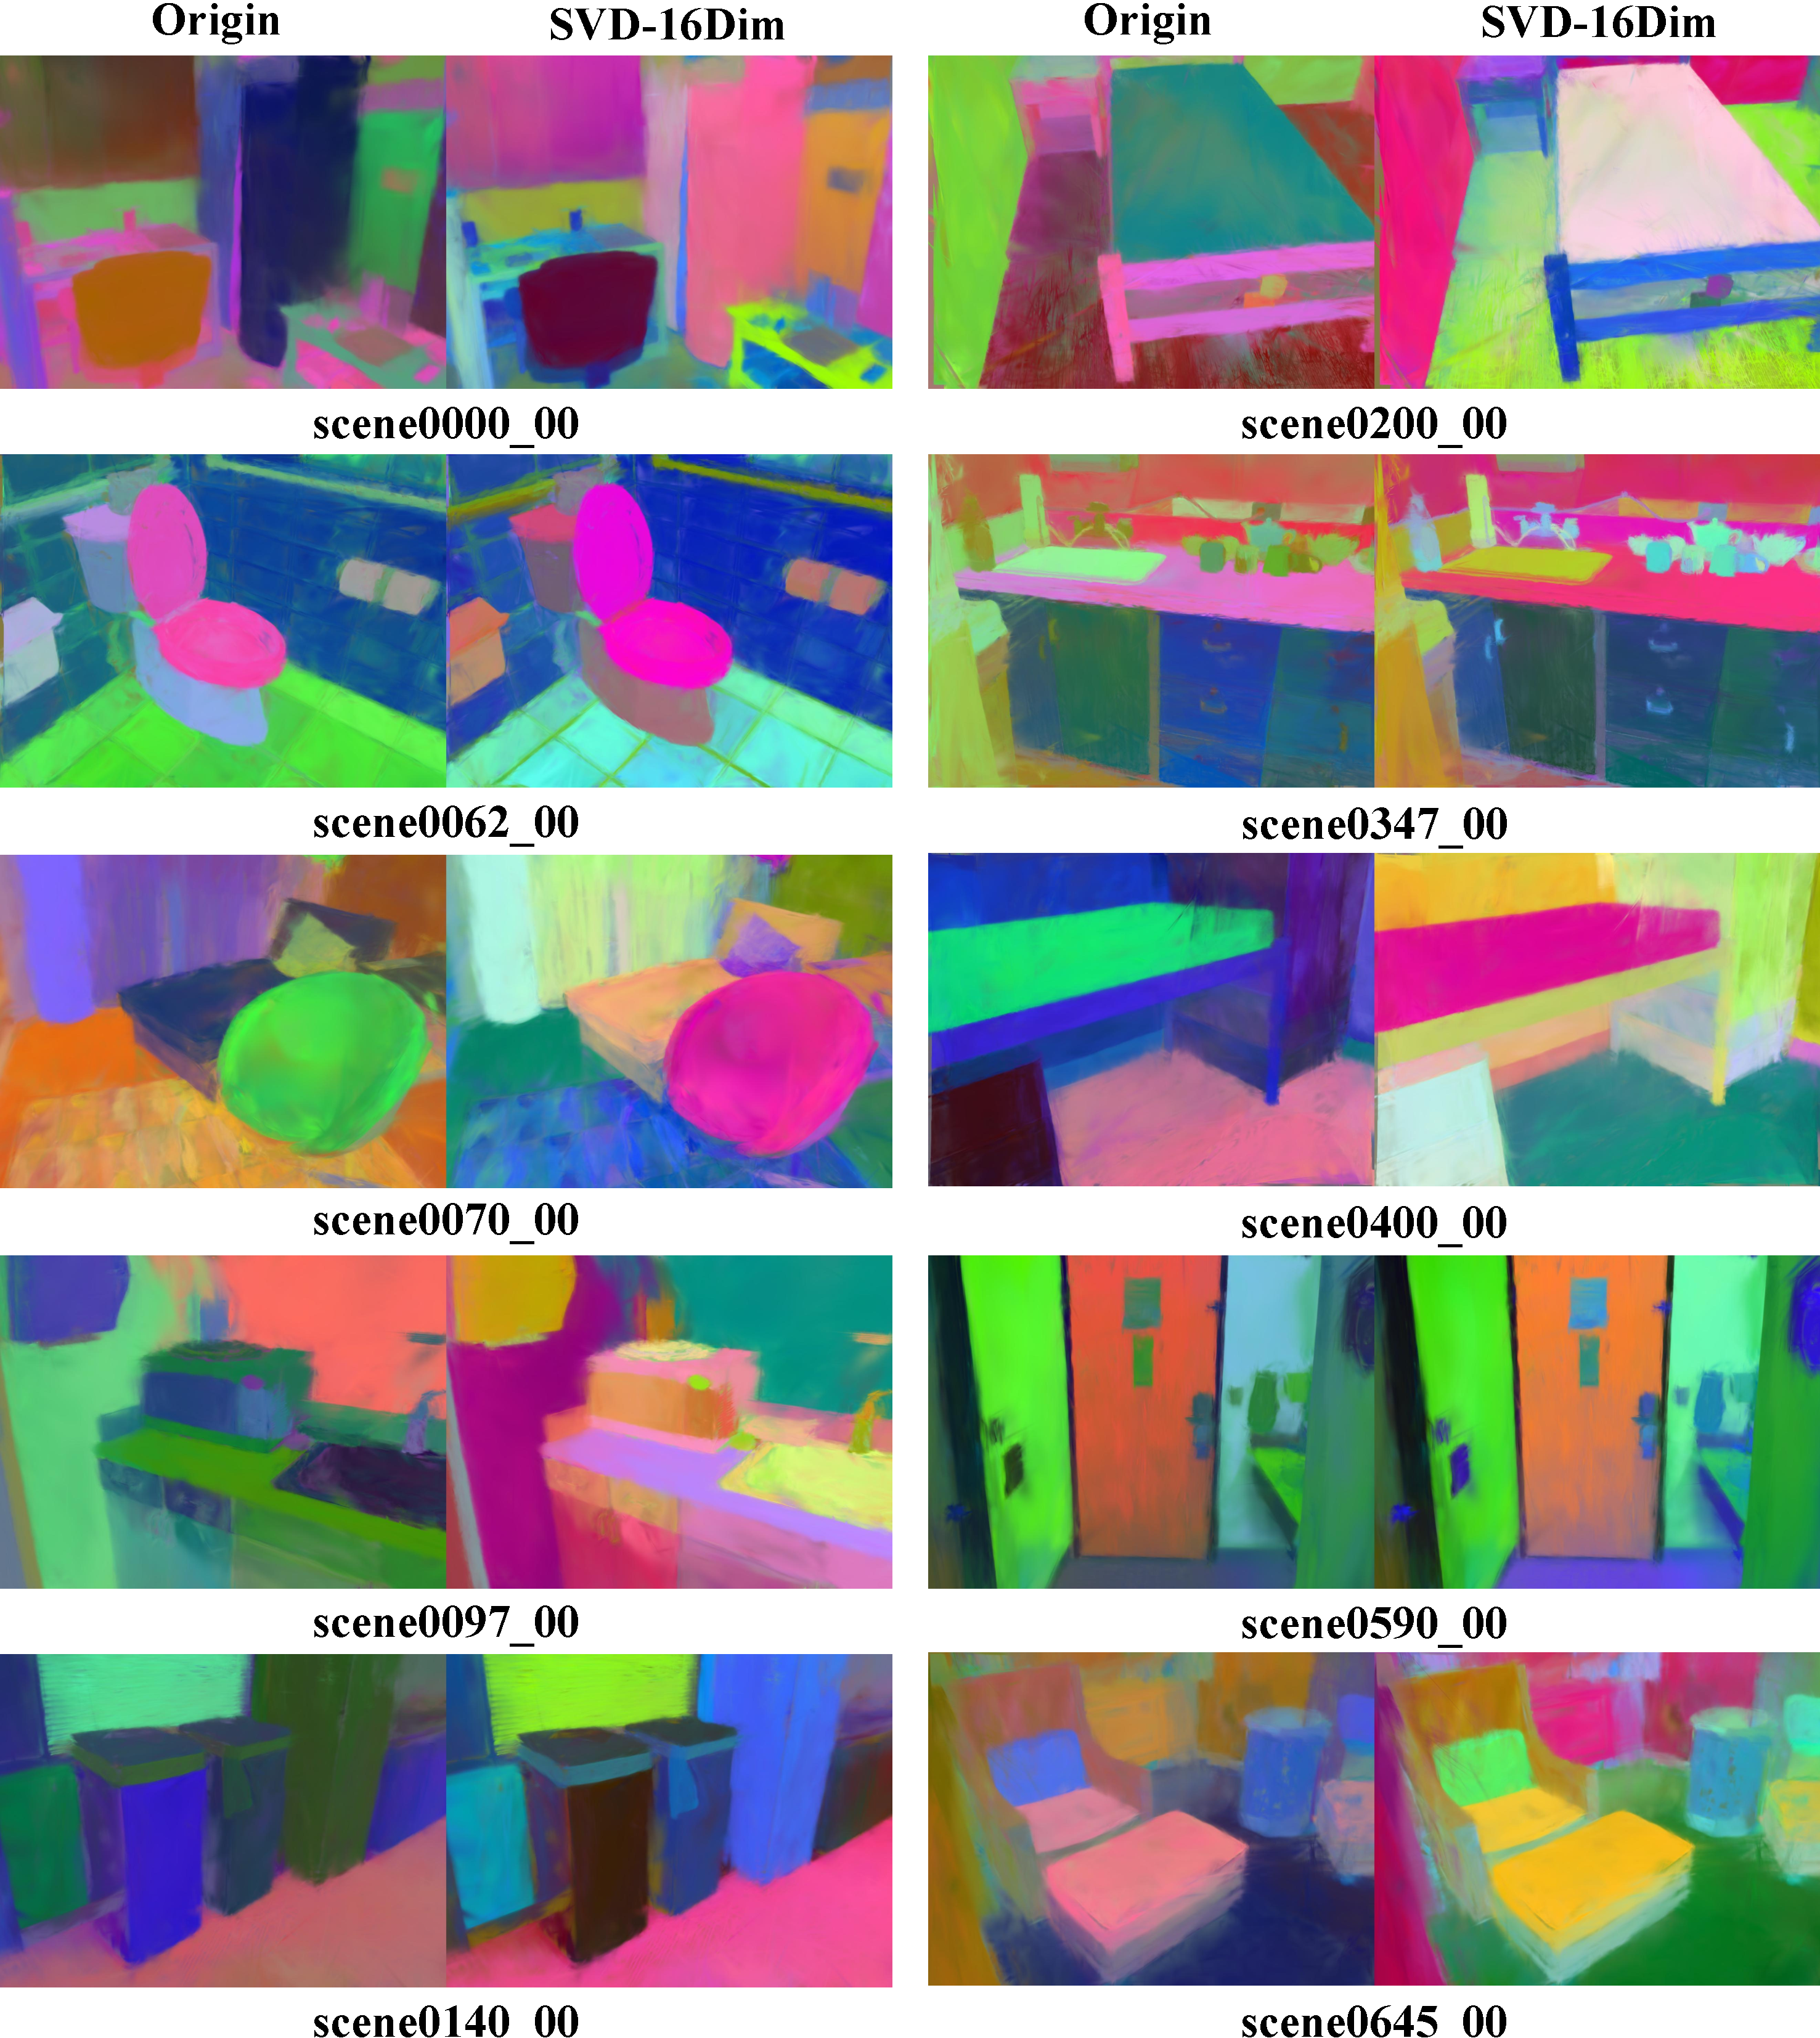
\includegraphics[width=\textwidth]{figs/SVDCompare.pdf}
  \caption{Visual comparison of feature maps on the ScanNet dataset before and after feature compression. Our method effectively preserves the original semantic information, although slight visual discrepancies exist compared to the original feature maps.}
  \label{fig:Visualize-Compare}
\end{figure}

% ---------------------------------------------------------------
% Bibliography
% ---------------------------------------------------------------
% Note: Usually supplementary material cites the same bib file as the main paper.
% Ensure your .bib file contains all references cited here.
